\subsection{Phân tích tập dữ liệu chỉ bao gồm các quan sát có cột "emailtotal" là giá trị null}

Quy trình phân tích tập dữ liệu chỉ bao gồm các quan sát có cột "emailtotal" là giá trị null khá tương tự phân tích tập dữ liệu chỉ bao gồm các quan sát có cột "emailtotal" không phải giá trị null.

\begin{figure}[H]
    \centering
    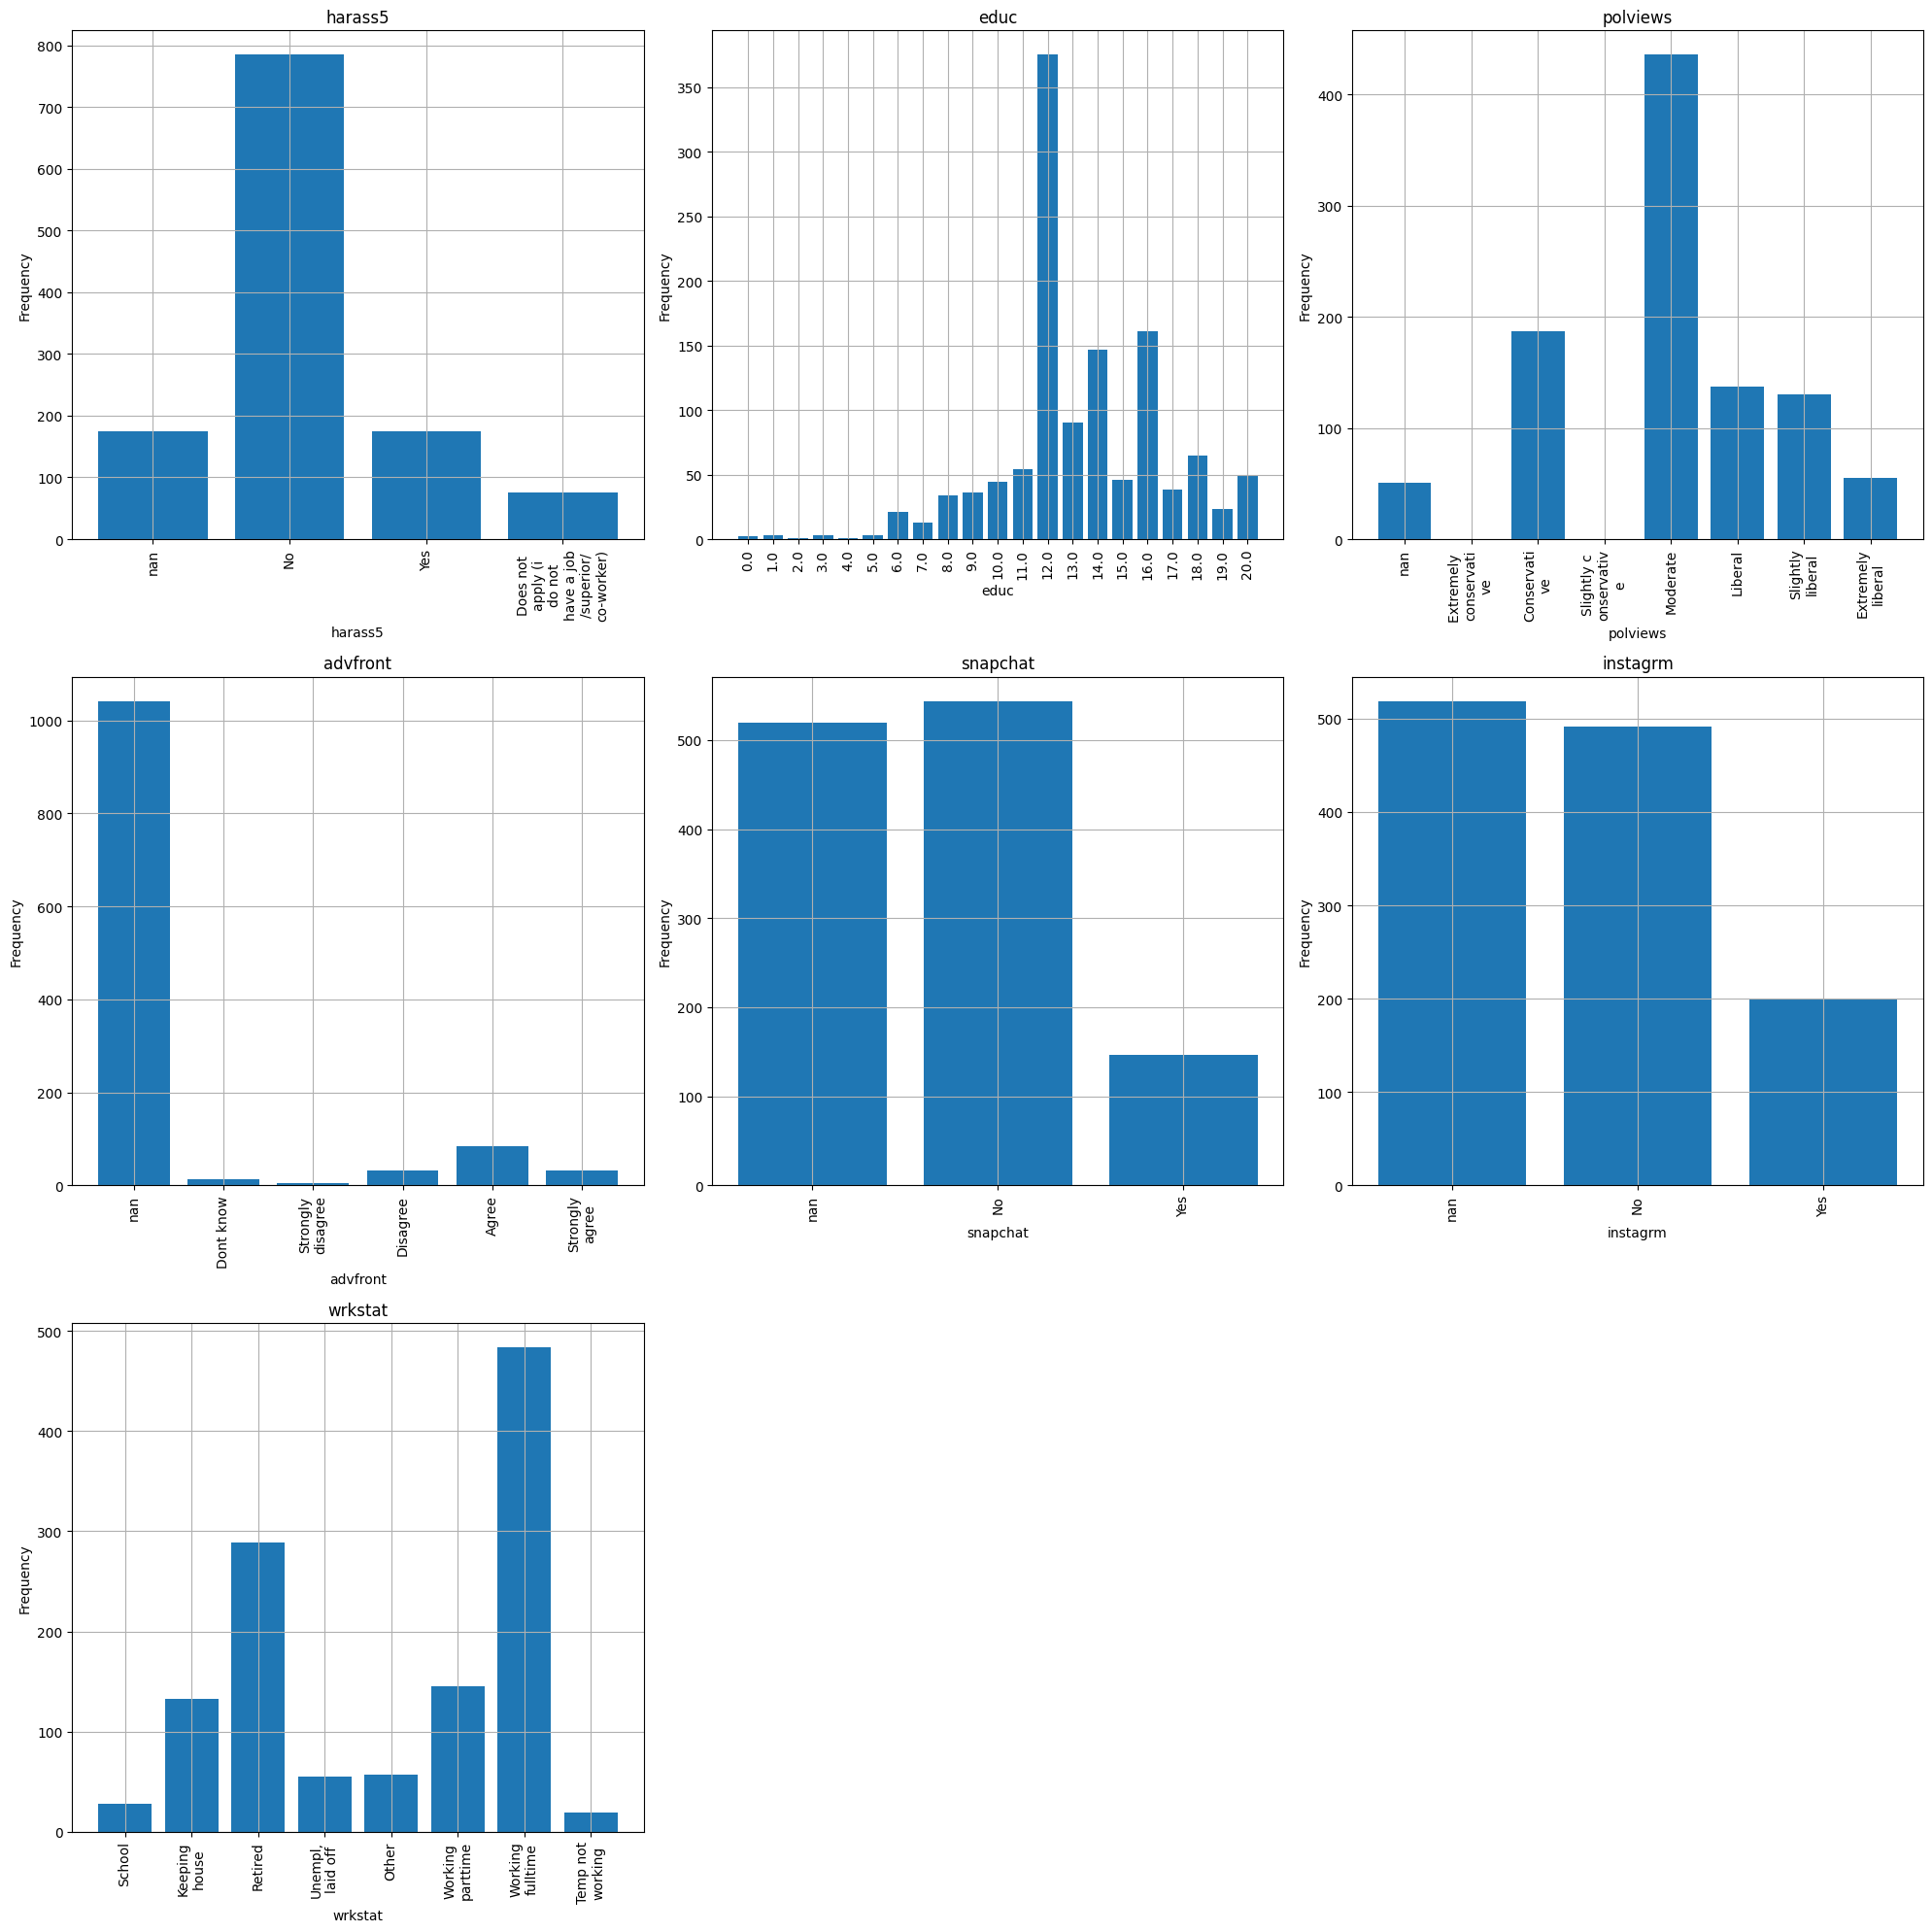
\includegraphics[width=0.6\textwidth]{figures/Thanh/Data_Analysis/With_null_frequency_of_unique_values_of_columns.png}
    \caption{Tần suất của từng giá trị của từng cột trong tập dữ liệu chỉ bao gồm các quan sát có cột "emailtotal" là giá trị null}
    \label{fig:With_null_frequency_of_unique_values_of_columns}
\end{figure}

Hình \ref{fig:With_null_frequency_of_unique_values_of_columns} cho biết tần suất của từng giá trị của từng cột trong tập dữ liệu chỉ bao gồm các quan sát có cột "emailtotal" là giá trị null.
Cột "harass5" có một lượng rất lớn các quan sát có giá trị là No.
Các quan sát có giá trị null giảm đi đáng kể.
Cột "educ" đa số các quan sát có học vấn từ 12 đến 16 năm.
Quan điểm chính trị đa số mọi người có quan điểm trung lập.
Sử dụng các mạng xã hội, đa số các quan sát là null hoặc No, tỷ lệ người có sử dụng hoặc không sử dụng snapchat hoặc instagrm tương đối bằng nhau.
Đa số mọi người ở tình trạng làm việc toàn thời gian (working fulltime).
Cột "advfront" đa số là giá trị là null.

\begin{figure}[H]
    \centering
    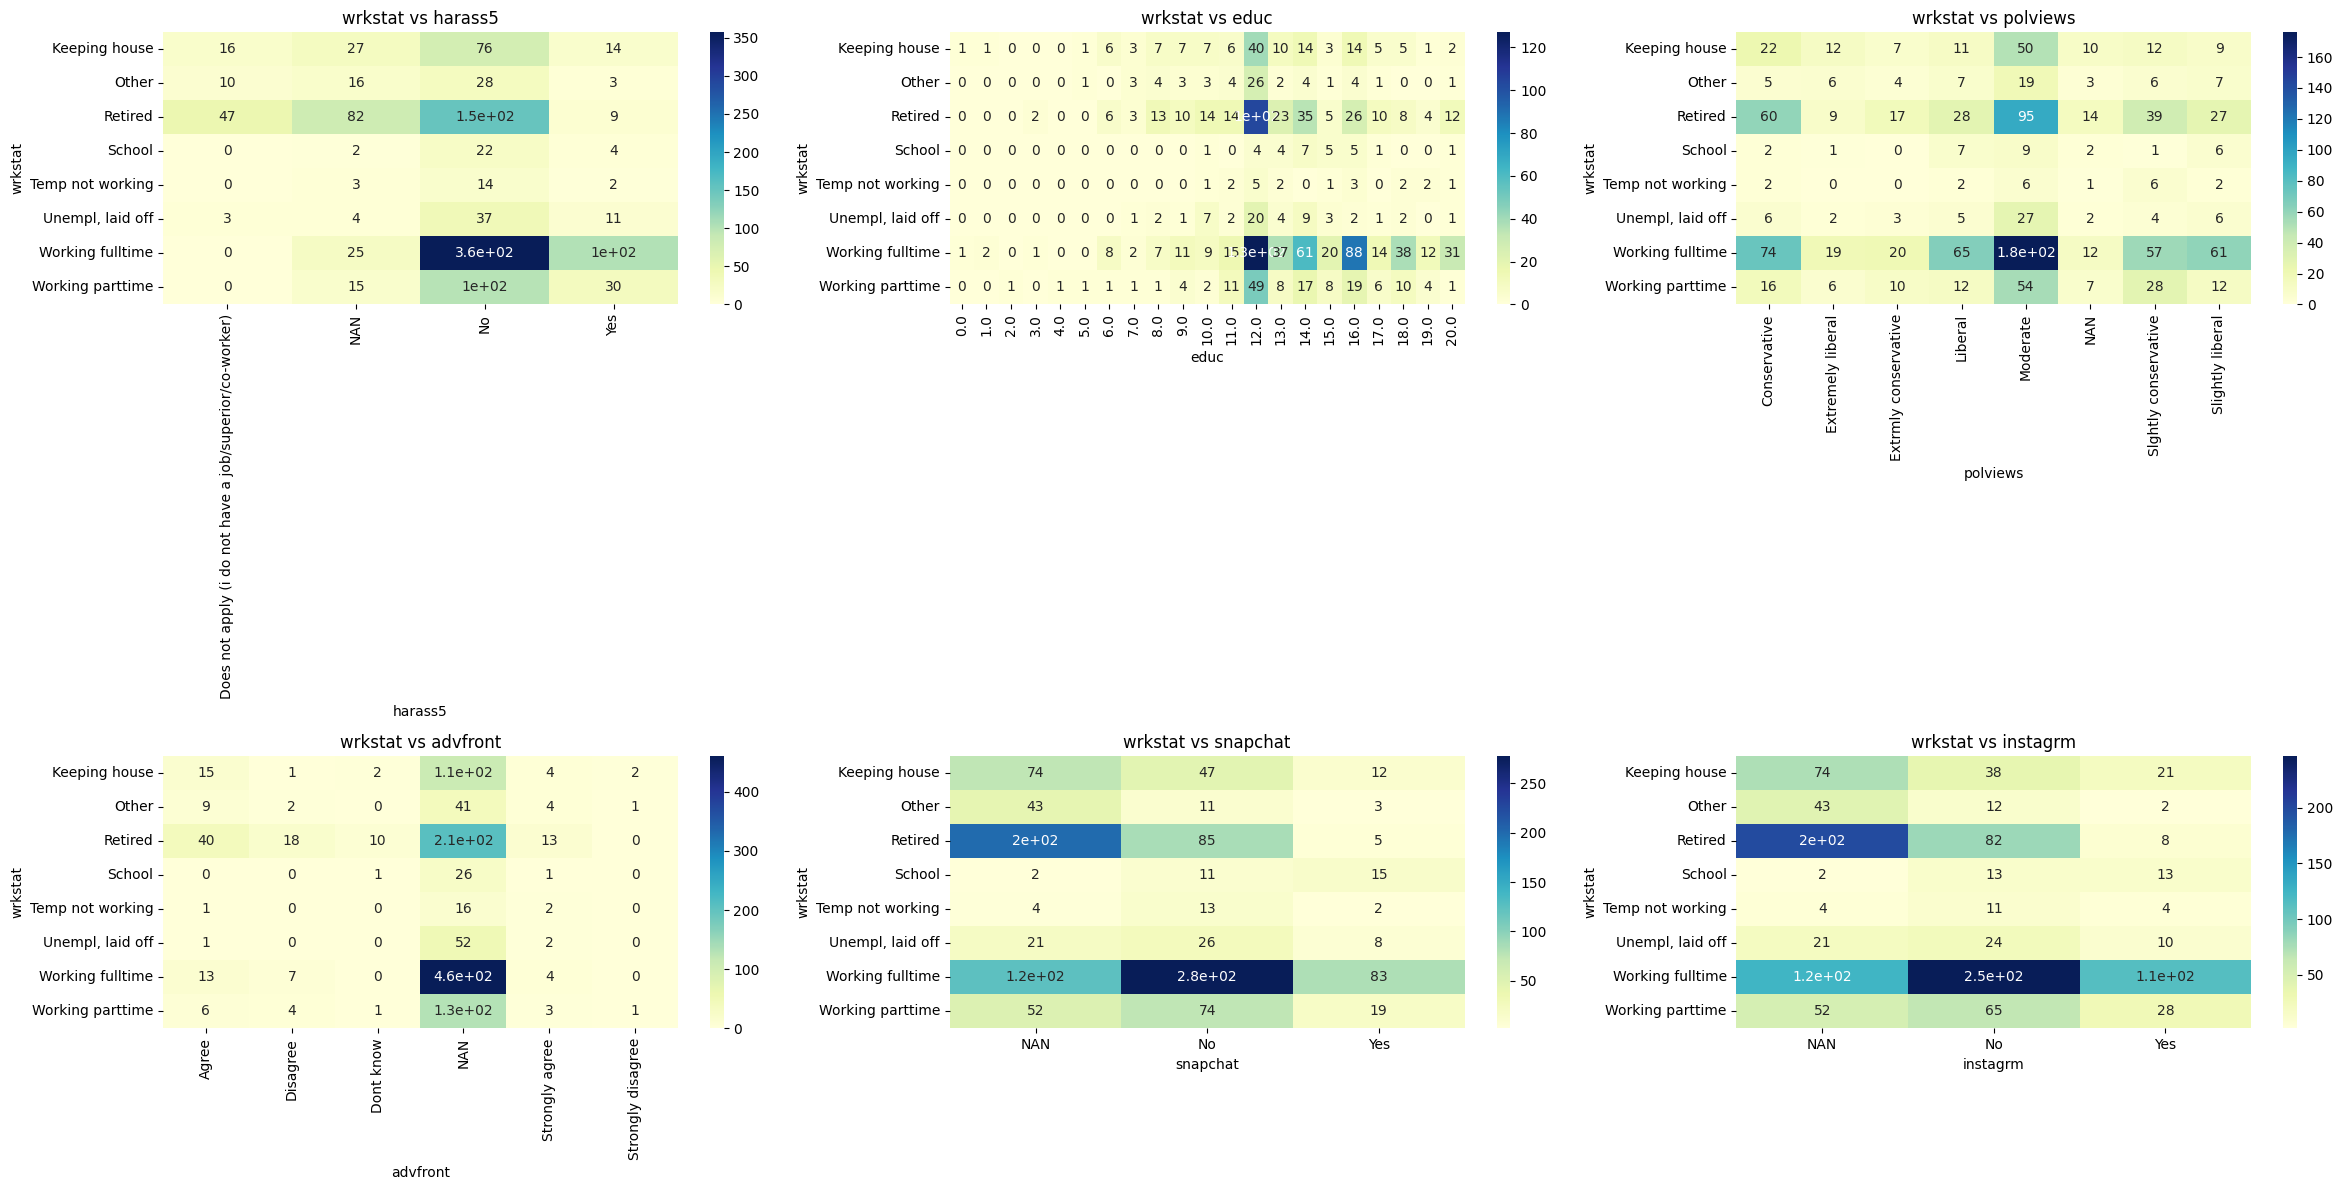
\includegraphics[width=0.8\textwidth]{figures/Thanh/Data_Analysis/With_null_cooccurrence_matrix_categorical_columns_vs_wrkstat.png}
    \caption{Ma trận đồng xuất hiện của các cột dạng phân loại với cột "wrkstat"}
    \label{fig:With_null_cooccurrence_matrix_categorical_columns_vs_wrkstat}
\end{figure}

Hình \ref{fig:With_null_cooccurrence_matrix_categorical_columns_vs_wrkstat} thể hiện các ma trận đồng xuất hiện của các cột dạng phân loại với cột "wrkstat".
Ta nhận thấy đối với từng ma trận đồng xuất hiện, các ô tương ứng với vị trí trạng thái làm việc là toàn thời gian lớn hơn các ô ứng với trạng thái làm việc khác.
Còn tại các cột dạng phân loại, độ lớn các ô theo từng giá trị tương ứng với các cột khá giống với biểu đồ cột ở hình \ref{fig:With_null_frequency_of_unique_values_of_columns}.

\begin{figure}[H]
    \centering
    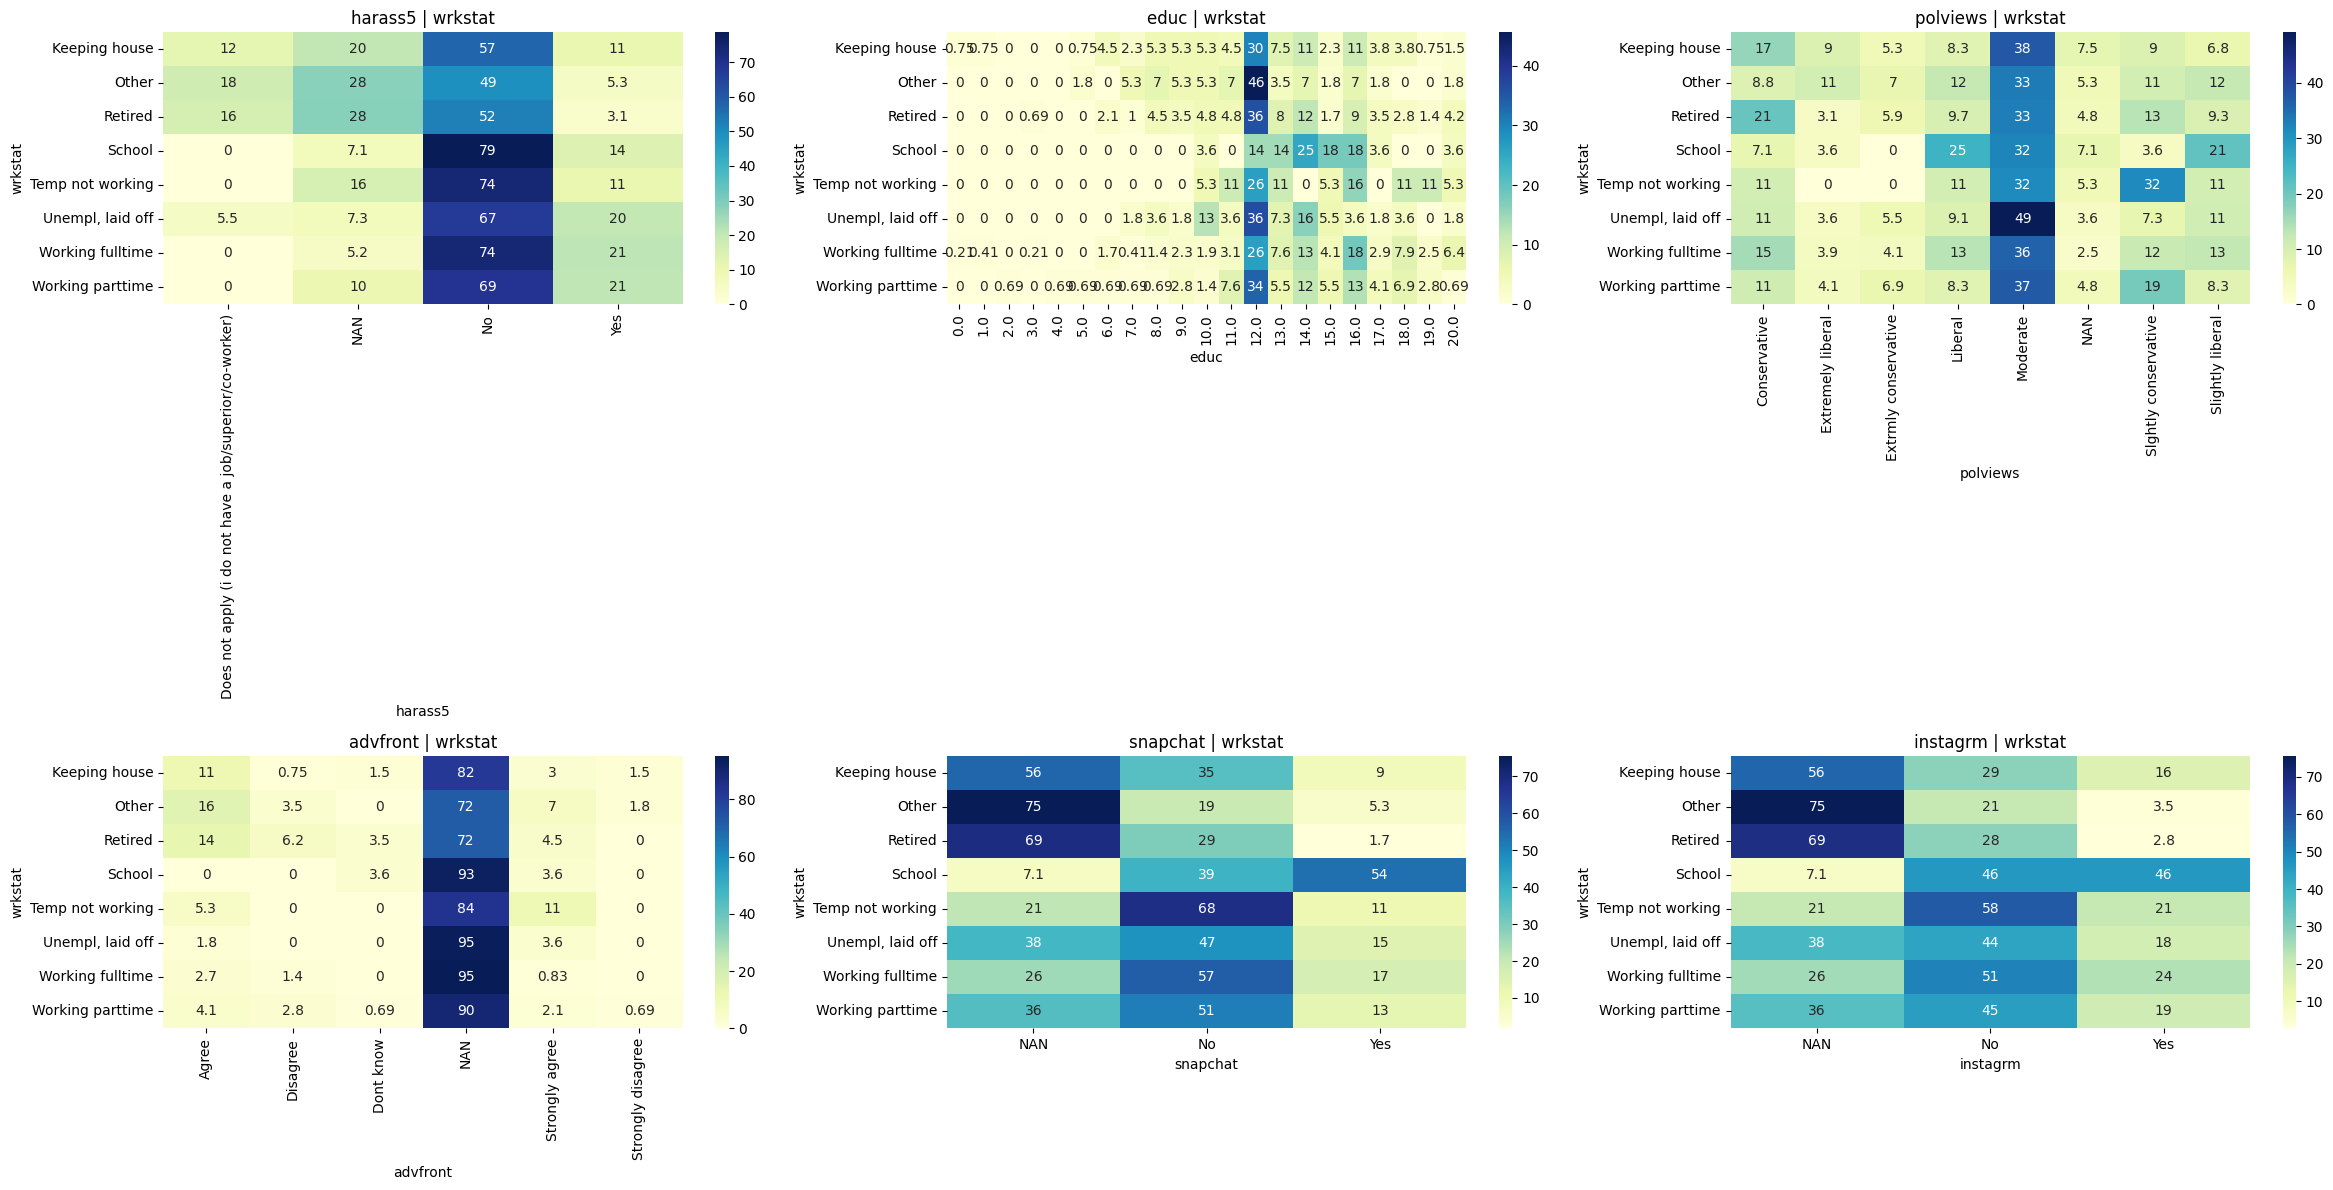
\includegraphics[width=0.6\textwidth]{figures/Thanh/Data_Analysis/With_null_percentage_matrix_categorical_columns_condition_on_wrkstat.png}
    \caption{Tính bảng tỷ lệ của các giá trị của các cột phân loại khi cố định từng giá trị của trường wrkstat}
    \label{fig:With_null_percentage_matrix_categorical_columns_condition_on_wrkstat}
\end{figure}

Hình \ref{fig:With_null_percentage_matrix_categorical_columns_condition_on_wrkstat} cho biết tỷ lệ có điều kiện của các cột dạng phân loại lấy điều kiện trên cột wrkstat.
Ta nhận thấy độ lớn các ô theo từng giá trị tương ứng với các cột khá giống với biểu đồ cột ở hình \ref{fig:With_null_frequency_of_unique_values_of_columns}.

\begin{figure}[H]
    \centering
    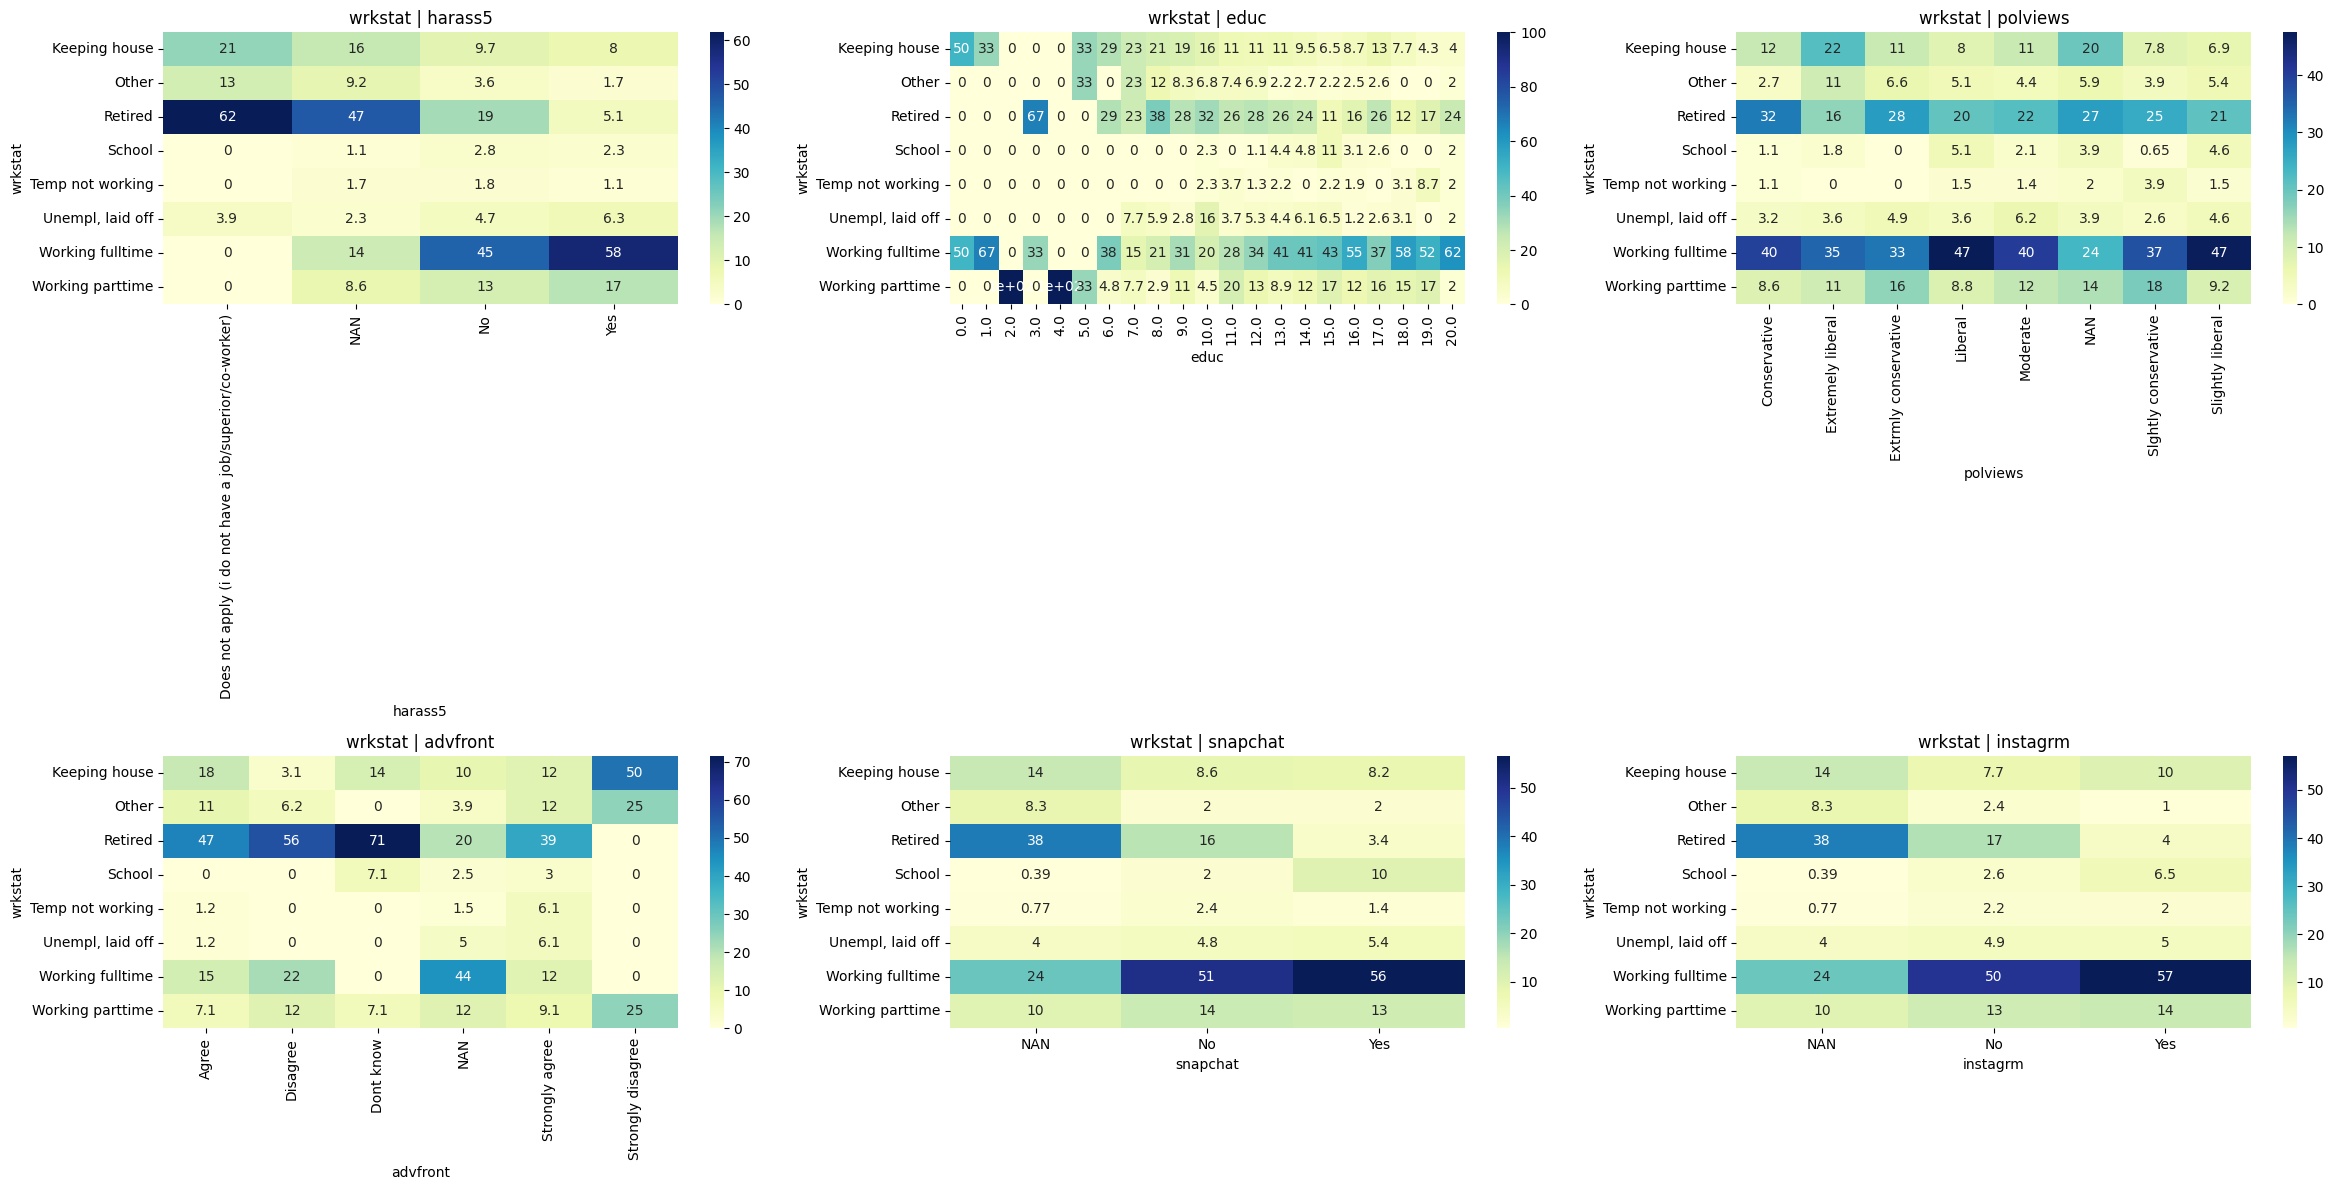
\includegraphics[width=0.6\textwidth]{figures/Thanh/Data_Analysis/With_null_percentage_matrix_categorical_wrkstat_condition_on_columns.png}
    \caption{Tỷ lệ của các giá trị của cột wrkstat khi cố định từng giá trị của các cột dạng phân loại}
    \label{fig:With_null_percentage_matrix_categorical_wrkstat_condition_on_columns}
\end{figure}

Hình \ref{fig:With_null_percentage_matrix_categorical_wrkstat_condition_on_columns} biểu diễn Tỷ lệ của các giá trị của cột wrkstat khi cố định từng giá trị của các cột dạng phân loại.
Ta nhận thấy ứng với mỗi giá trị của các cột khác về cơ bản tỷ lệ người đang trong trạng thái làm việc toàn thời gian có tỷ lệ cao nhất trừ một số trường hợp đặc biệt như người không tham gia lao động thì tỷ lệ người đã nghỉ hưu là cao nhất.
Nhưng trong trường hợp đặc biệt nếu các cột snapchat hoặc instagrm có giá trị là null thì đa số các quan sát trong trạng thái làm việc là đã nghỉ hưu.

\begin{table}[ht]
    \centering
    \begin{tabular}{|l|l|}
    \hline
    Cột & p-value \\
    \hline
    harass5 & $8.64 \times 10^{-43}$ \\
    \hline
    educ & $9.25 \times 10^{-6}$ \\
    \hline
    polviews & $0.0104$ \\
    \hline
    advfront & $9.090 \times 10^{-14}$ \\
    \hline
    snapchat & $1.96 \times 10^{-42}$ \\
    \hline
    instagrm & $3.13 \times 10^{-38}$ \\
    \hline
    \end{tabular}
    \caption{Bảng chisquare test kiểm tra tính độc lập của từng cột dạng biến phân loại với cột trạng thái làm việc wrkstat}
    \label{tab:With_null_chisquare_test}
\end{table}

Ta sử dụng kiểm định chisquare để kiểm tra tính độc lập của từng cột dạng biến phân loại với cột trạng thái làm việc wrkstat.
Các giá trị p-value được thể hiện ở trên bảng \ref{tab:With_null_chisquare_test}.
Ta nhận thấy tất cả các giá trị p-value tương ứng với từng cặp giữa các cột dạng biến phân loại và cột trạng thái làm việc đều nhỏ hơn 0.05.
Vậy với mức ý nghĩa 0.05, từng cột dạng biến phân loại không độc lập với cột trạng thái làm việc.

\begin{figure}[H]
    \centering
    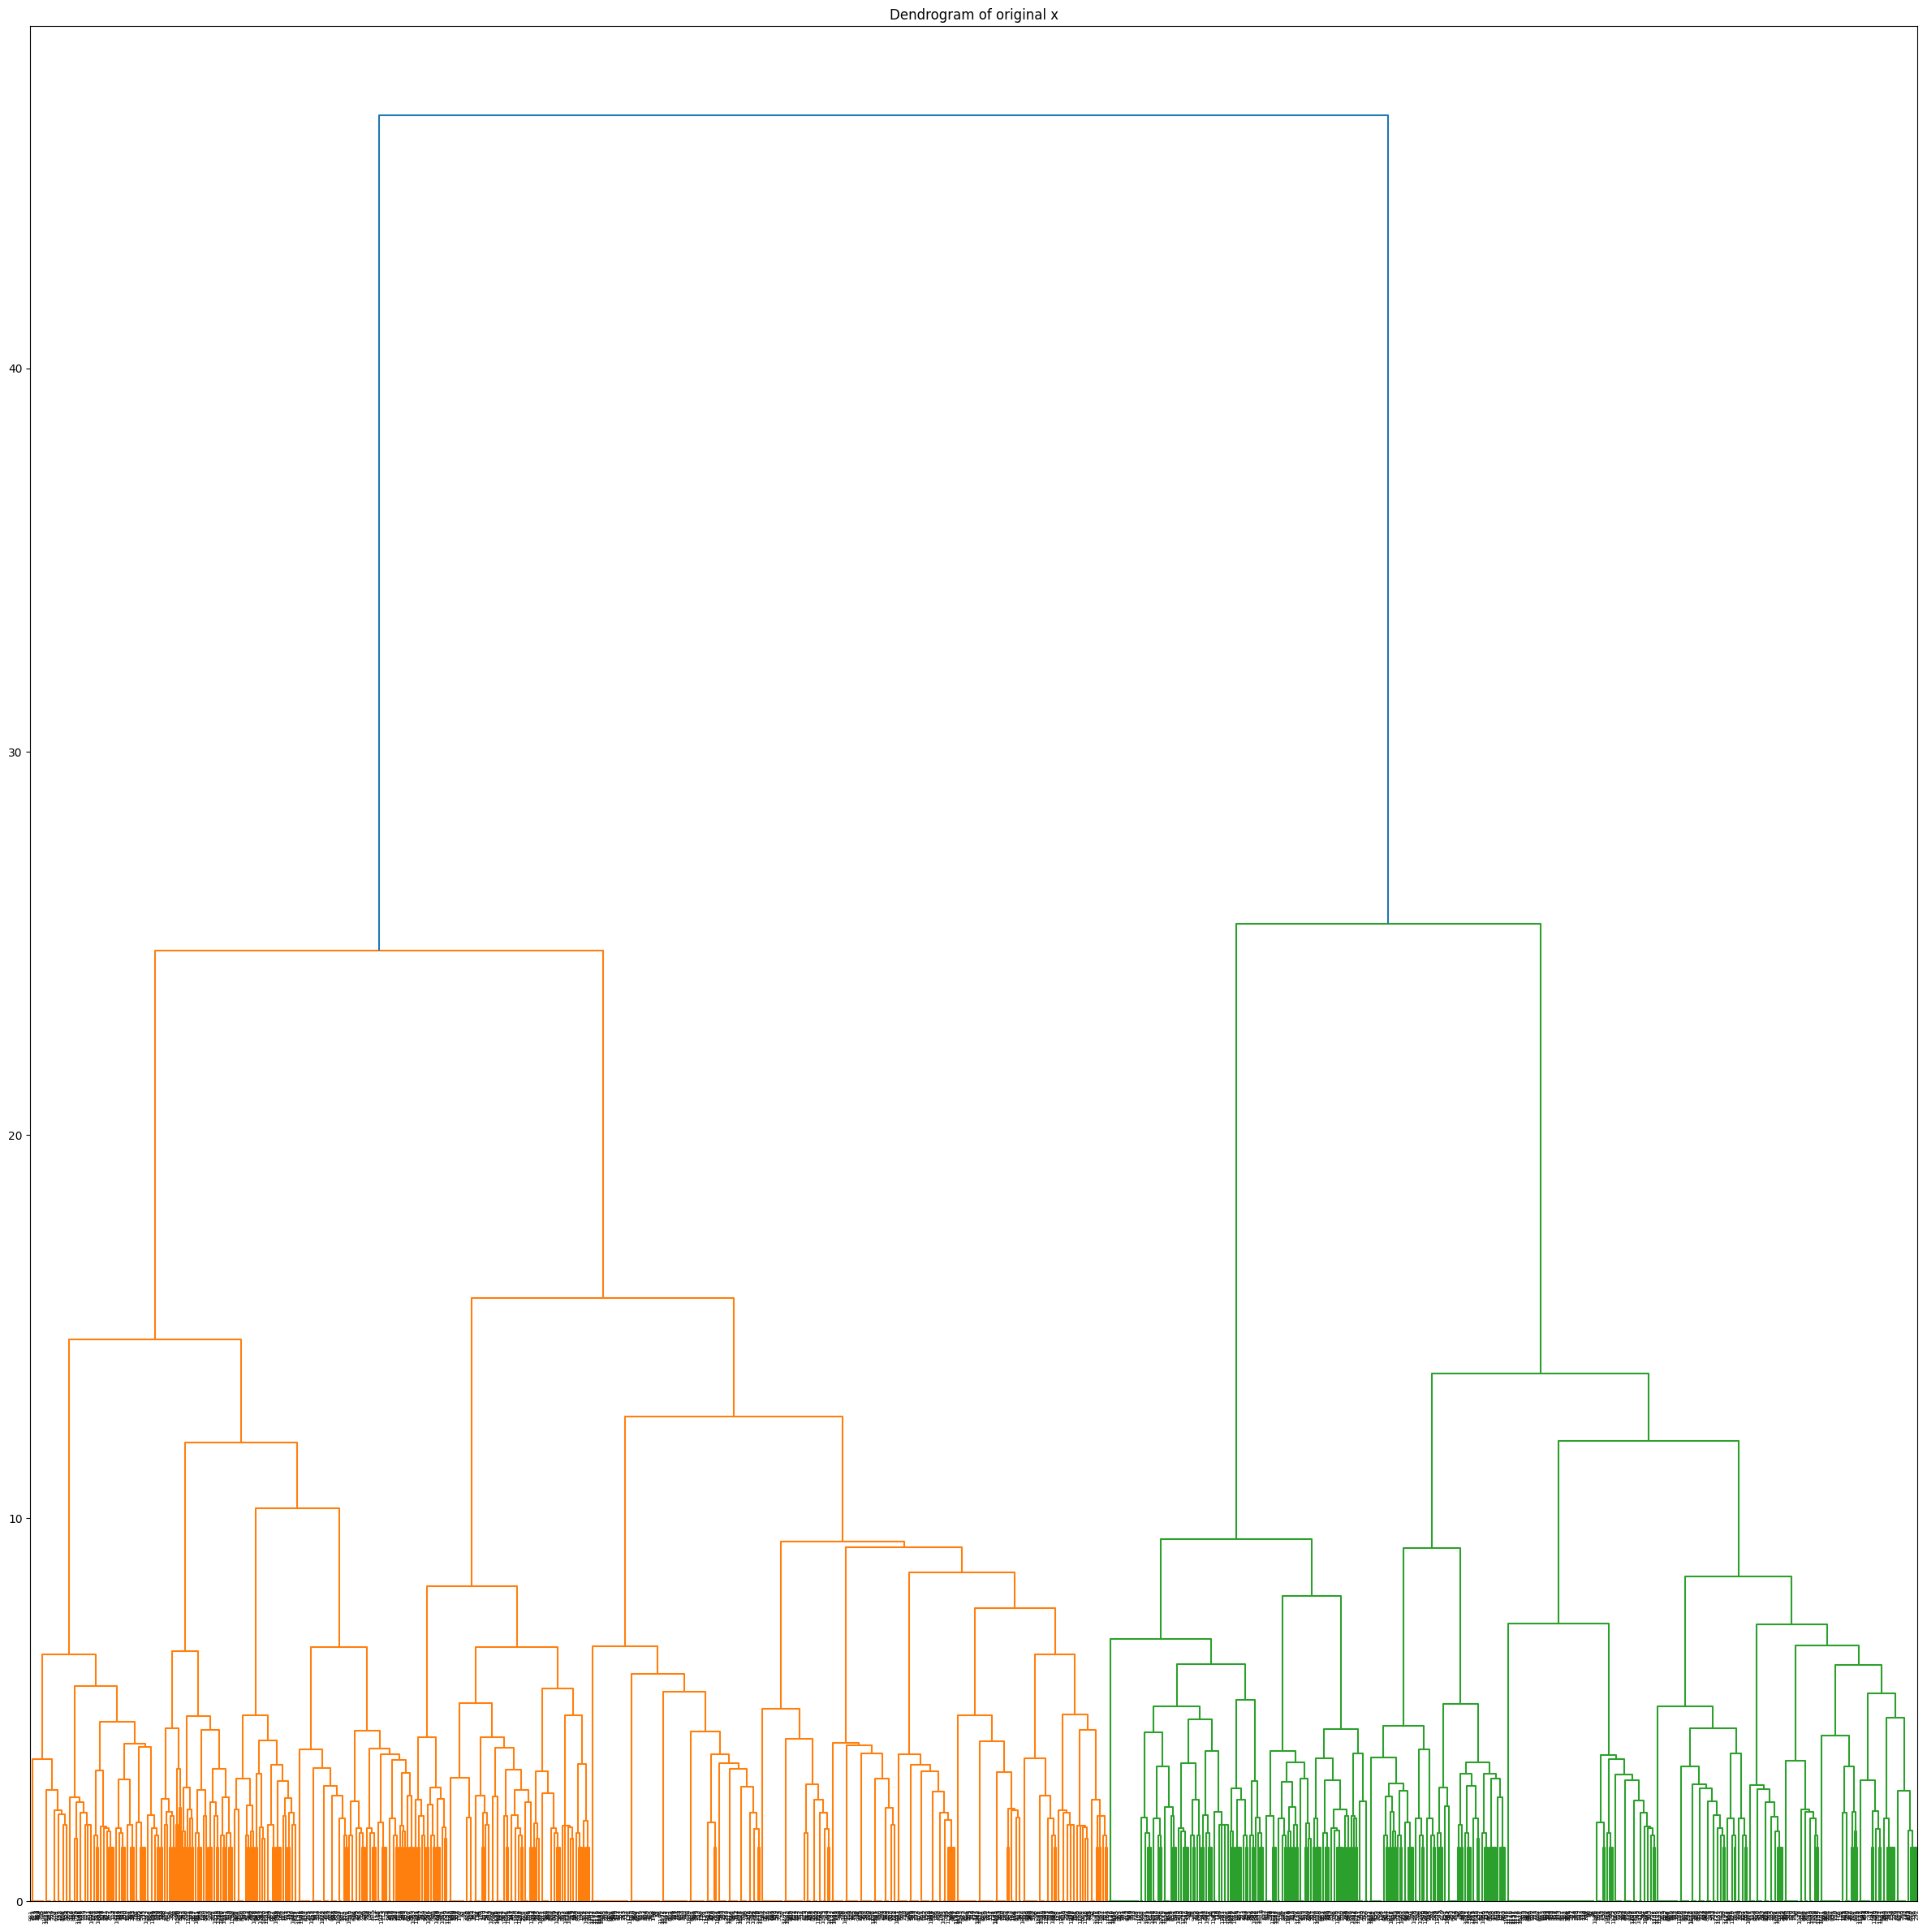
\includegraphics[width=0.6\textwidth]{figures/Thanh/Data_Analysis/With_null_dendrogram_original_features.png}
    \caption{Dendrogram của tập dữ liệu với biểu diễn là các vector gốc ban đầu}
    \label{fig:With_null_dendrogram_original_features}
\end{figure}

Để biểu diễn dữ liệu các quan sát thành các vector.
Đối với các cột dạng biến phân loại là harass5, educ, polviews, advfront, snapchat, instagrm ta sử dụng phương pháp one-hot encoding.
Với các giá trị null ta xem như có giá trị là Unknown.
Vector cho mỗi quan sát thu được từ phương pháp trên ta gọi là "vector gốc ban đầu".

Hình \ref{fig:With_null_dendrogram_original_features} thể hiện dendrogram của tập dữ liệu với biểu diễn là các vector gốc ban đầu.
Nhìn sơ bộ, ta nhận thấy có 2 nhóm (cụm) lớn.

\begin{figure}[H]
    \centering
    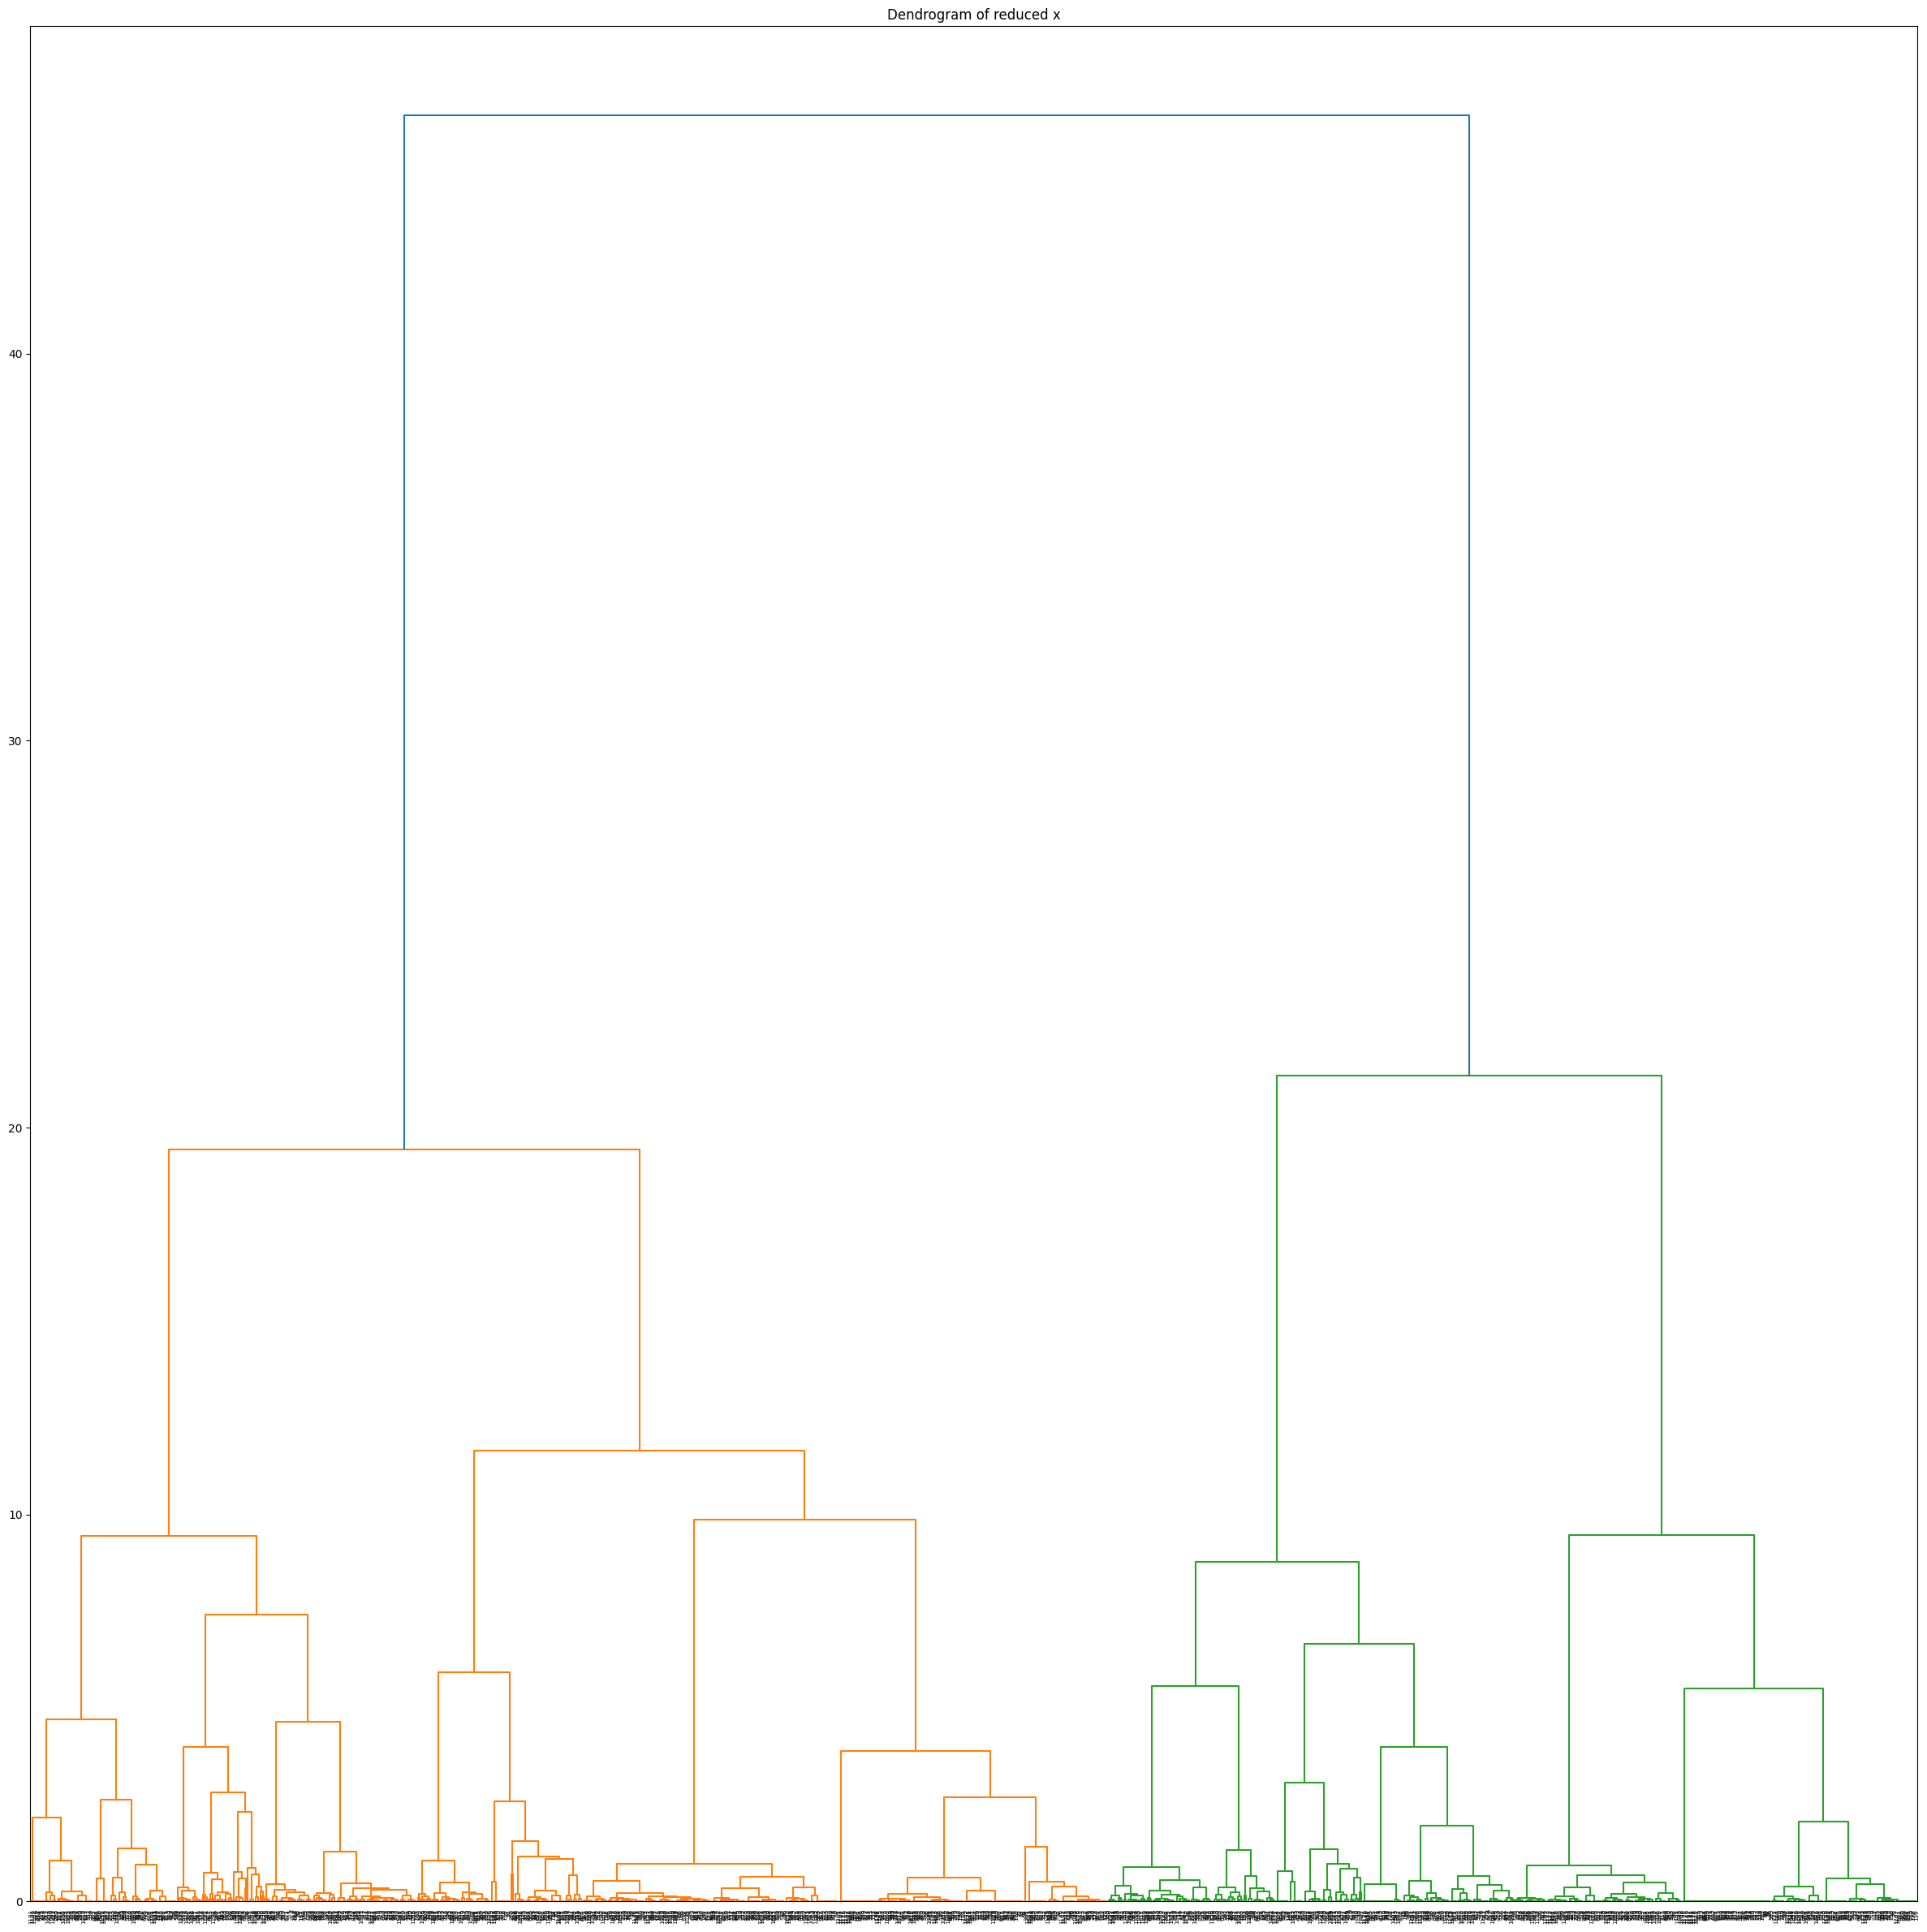
\includegraphics[width=0.6\textwidth]{figures/Thanh/Data_Analysis/With_null_dendrogram_PCA_features.png}
    \caption{Dendrogram của tập dữ liệu với biểu diễn là các vector thu được từ việc phân tích thành phần chính bằng thuật toán PCA}
    \label{fig:With_null_dendrogram_PCA_features}
\end{figure}

Ngoài ra ta cũng có thể biểu diễn các quan sát bằng cách phân tích các thành phần chính dùng thuật toán PCA từ các vector gốc ban đầu biểu diễn các quan sát.
Hình \ref{fig:With_null_dendrogram_PCA_features} biểu diễn dendrogram của tập dữ liệu với biểu diễn của các quan sát là các vector đã được phân tích thành phần chính từ vector gốc ban đầu.
Ta nhận thấy vẫn có 2 nhóm (cụm) lớn. Dendrogram được xây dựng từ tập dữ liệu mà các quan sát được biểu diễn từ phân tích thành phần chính không khác nhiều so với dendrogram được xây dựng từ các vector gốc ban đầu.

Ta sẽ phân tích histogram của các thành phần chính.
Ta phân tích histogram 3 thành phần chính đầu tiên.

\begin{figure}[H]
    \centering
    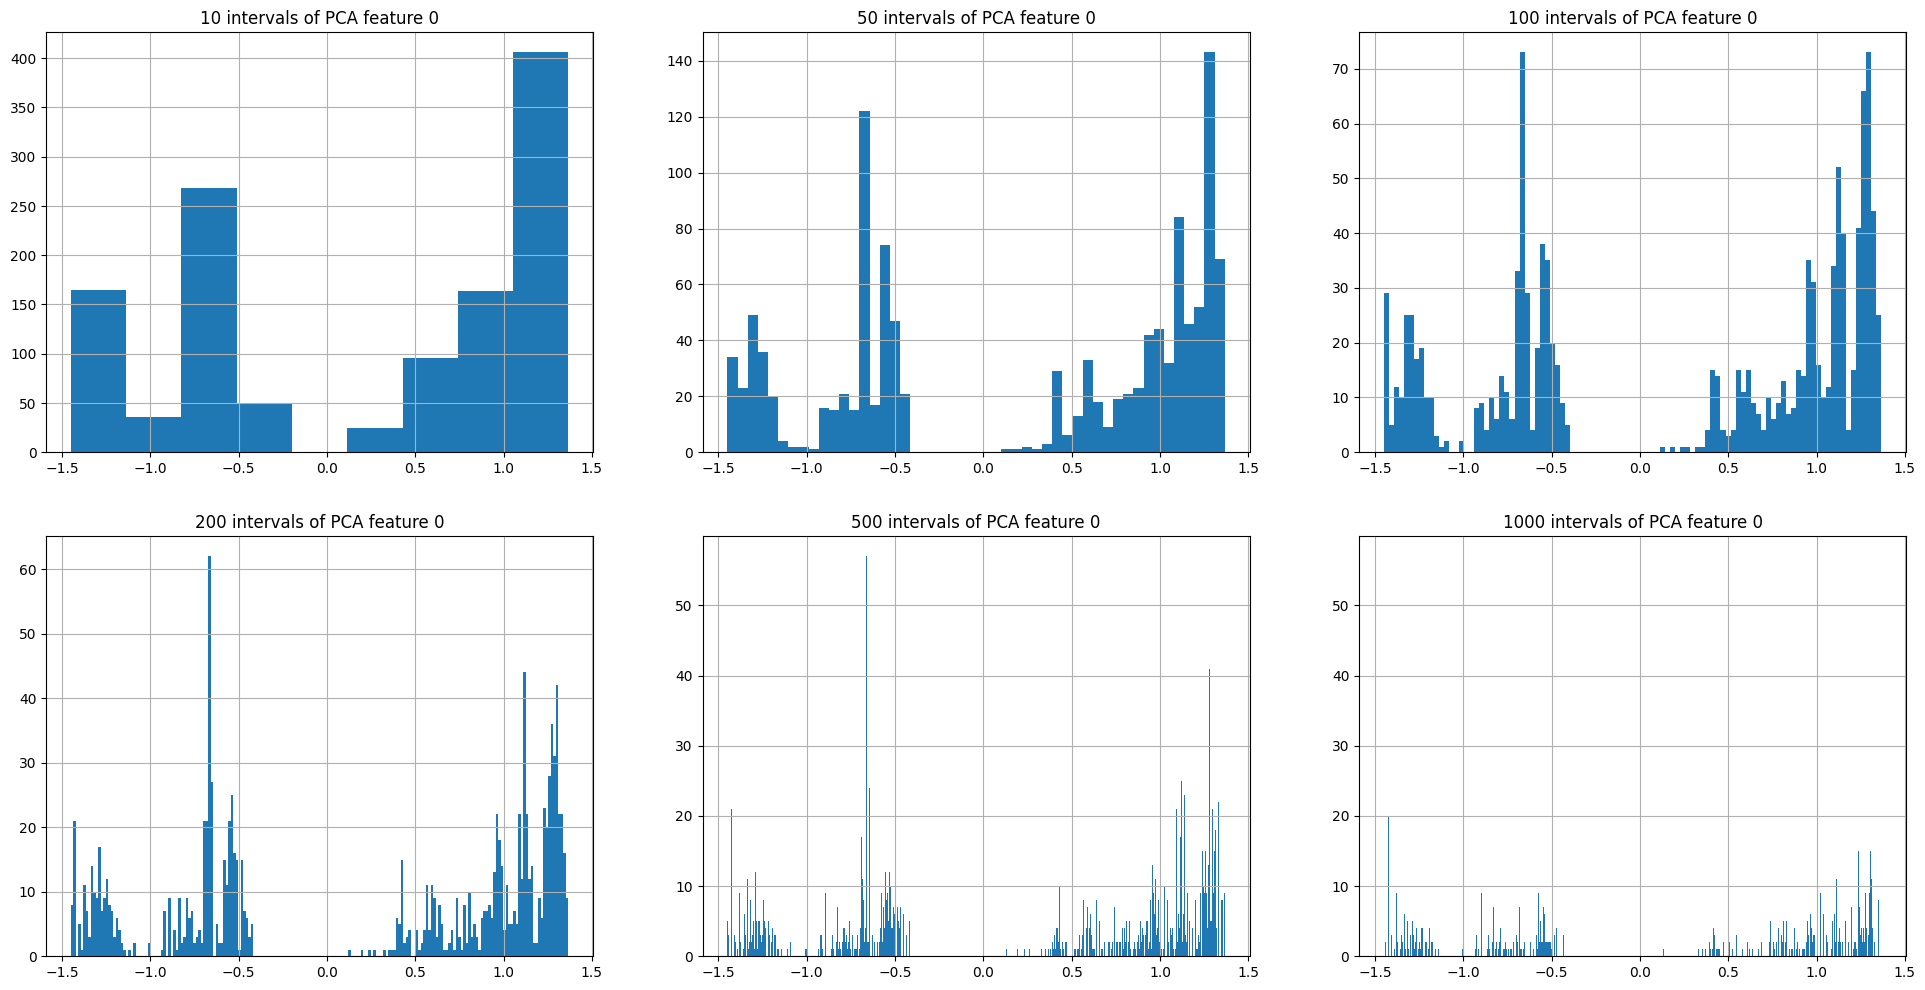
\includegraphics[width=0.75\textwidth]{figures/Thanh/Data_Analysis/With_null_histogram_PCA_feature_0.png}
    \caption{Histogram của thành phần chính thứ nhất}
    \label{fig:With_null_histogram_PCA_feature_0}
\end{figure}

Hình \ref{fig:With_null_histogram_PCA_feature_0} biểu diễn histogram ứng với độ lớn khác nhau của các bins khác nhau.
Ta nhận thấy histogram có 3 đỉnh gợi ý có 3 nhóm các quan sát khi nhìn từ thành phần chính thứ nhất.
Kết quả tương đối khác với dendrogram đã được biểu diễn ở các hình \ref{fig:With_null_dendrogram_original_features} và \ref{fig:With_null_dendrogram_PCA_features}.

\begin{figure}[H]
    \centering
    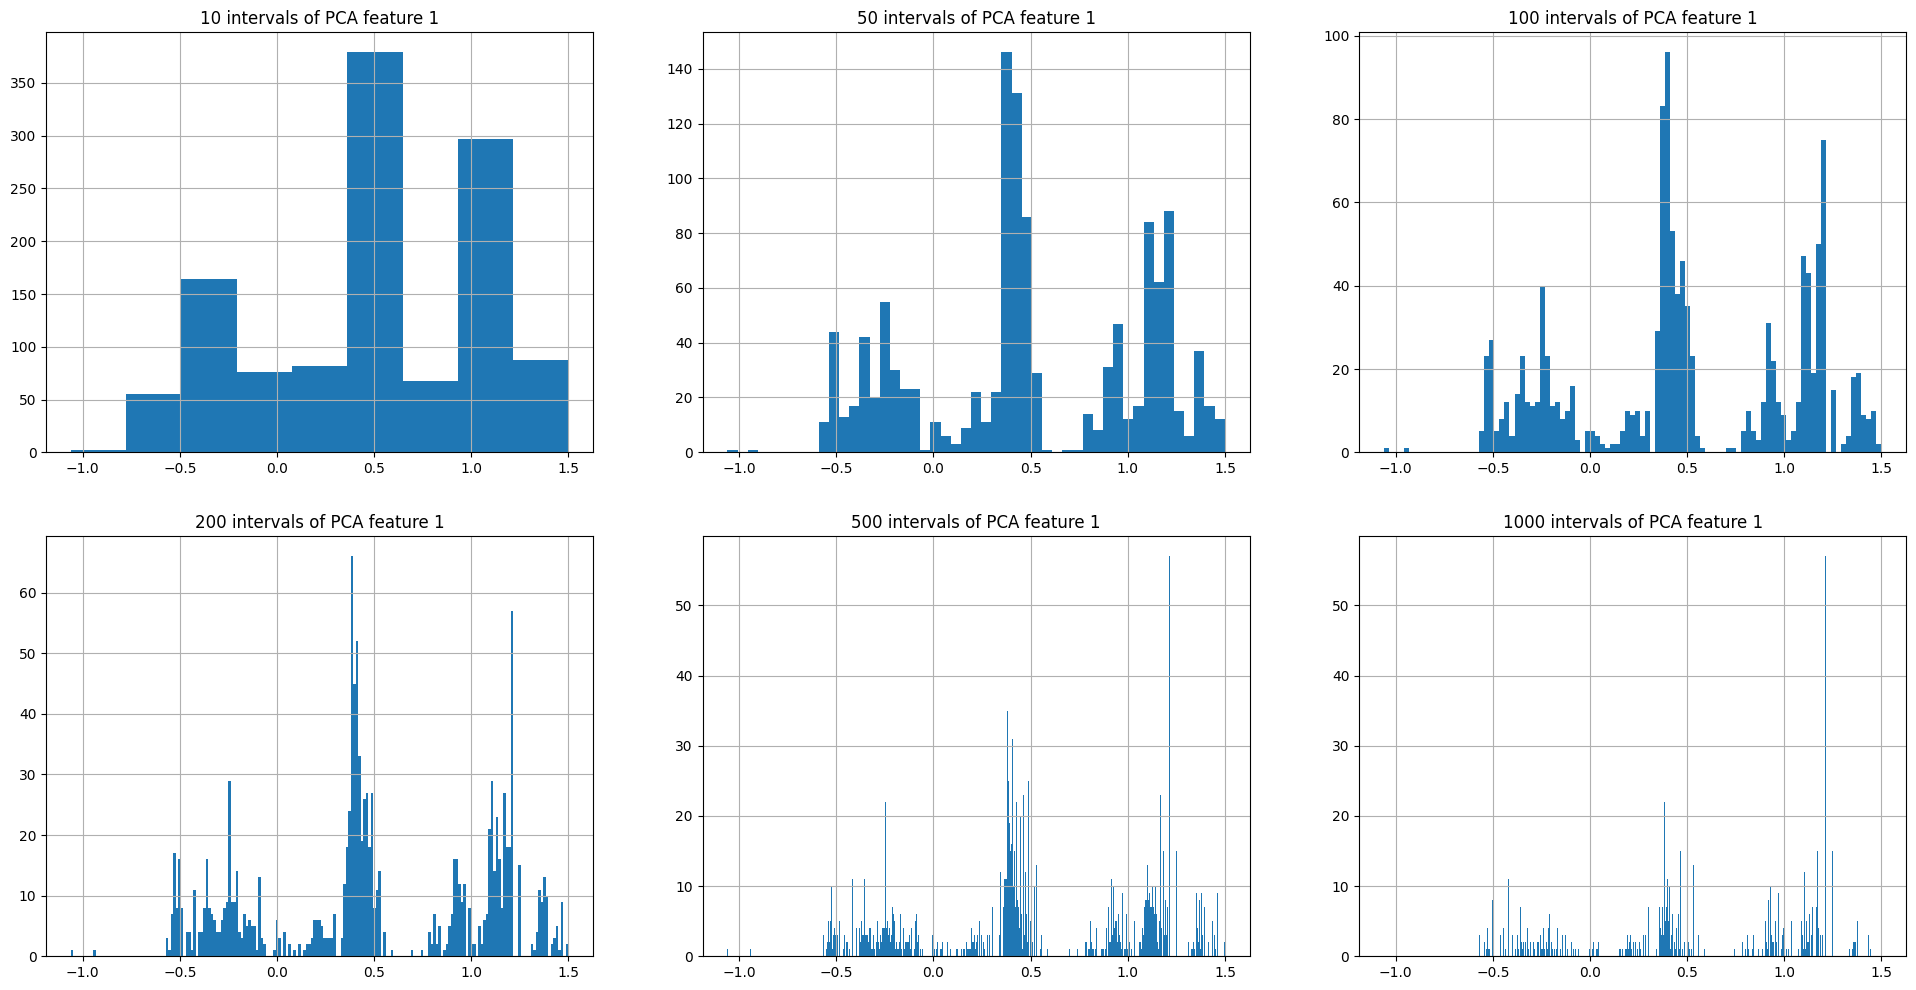
\includegraphics[width=0.75\textwidth]{figures/Thanh/Data_Analysis/With_null_histogram_PCA_feature_1.png}
    \caption{Histogram của thành phần chính thứ hai}
    \label{fig:With_null_histogram_PCA_feature_1}
\end{figure}

Hình \ref{fig:With_null_histogram_PCA_feature_1} biểu diễn histogram ứng với độ lớn khác nhau của các bins khác nhau của thành phần chính thứ hai.
Ta nhận thấy histogram có 3 nhóm lớn nếu nhìn từ thành phần chính thứ hai.

\begin{figure}[H]
    \centering
    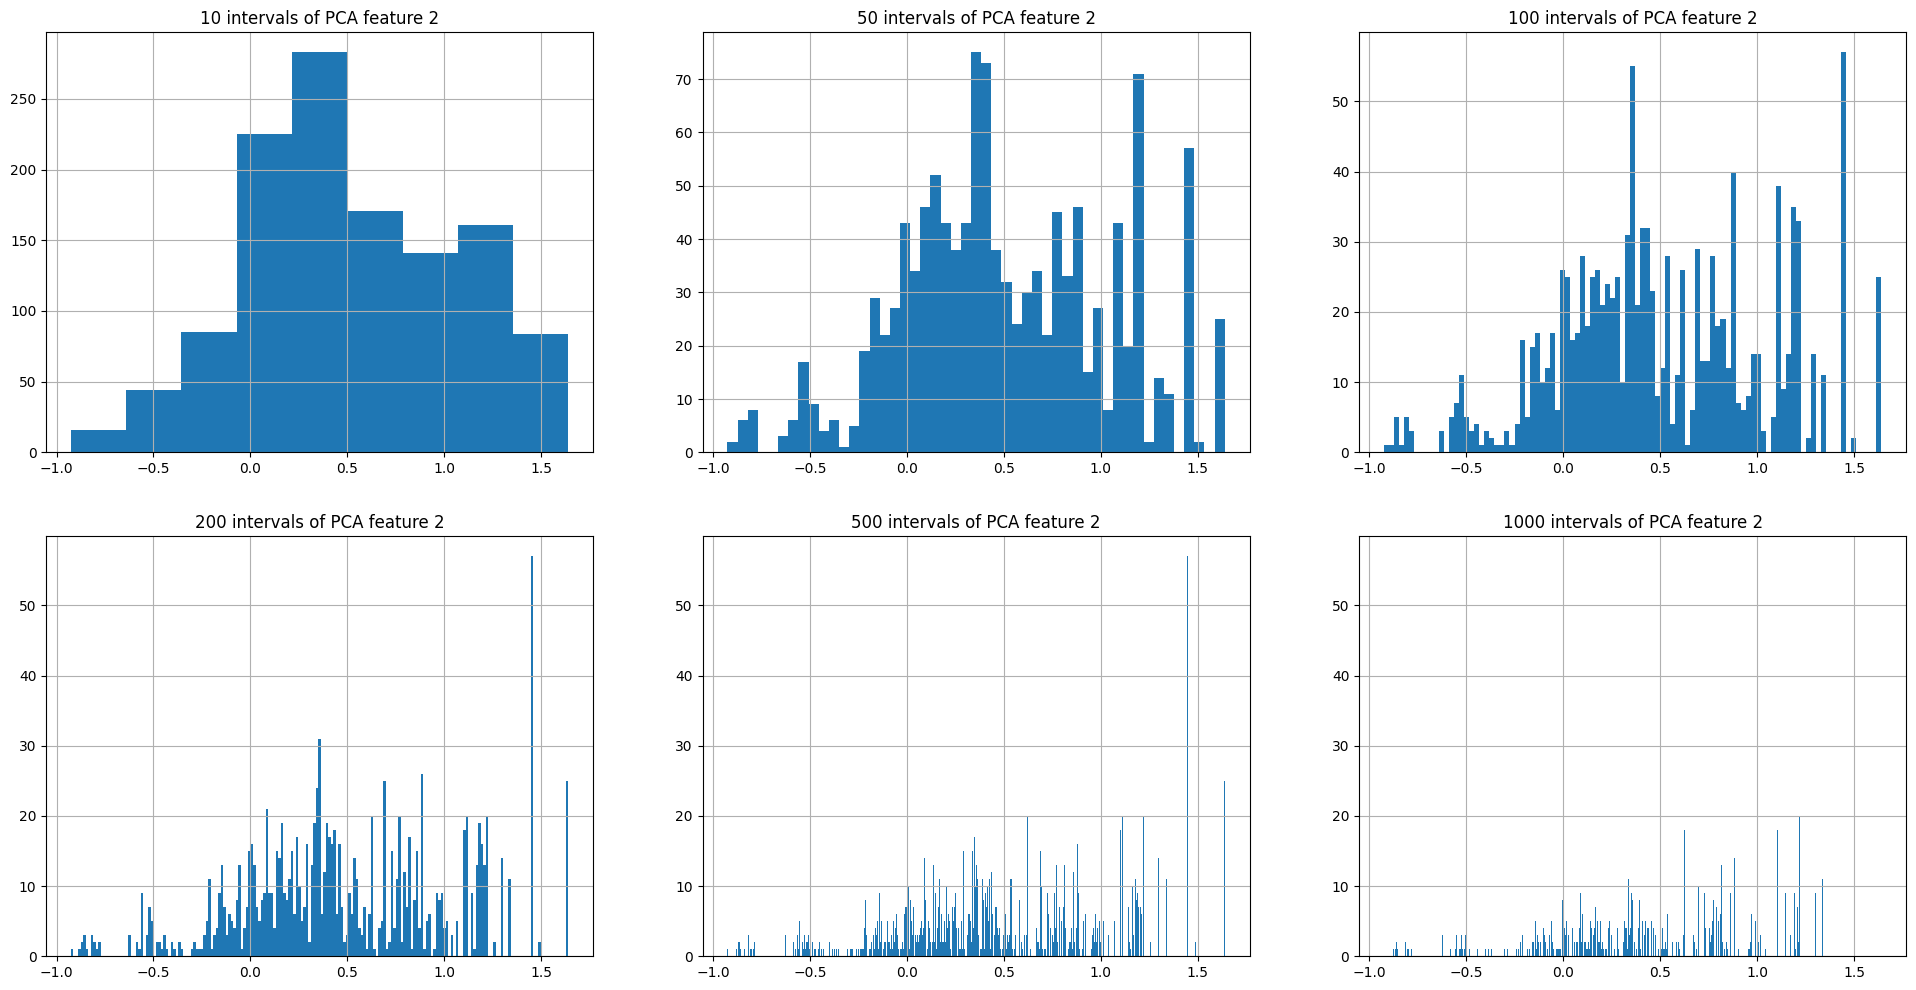
\includegraphics[width=0.75\textwidth]{figures/Thanh/Data_Analysis/With_null_histogram_PCA_feature_2.png}
    \caption{Histogram của thành phần chính thứ ba}
    \label{fig:With_null_histogram_PCA_feature_2}
\end{figure}

Hình \ref{fig:With_null_histogram_PCA_feature_2} biểu diễn histogram ứng với độ lớn khác nhau của các bins khác nhau của thành phần chính thứ ba.
Ta thấy có một đỉnh chính lớn nếu nhìn từ thành phần chính thứ ba.

Ta sẽ thử vẽ các histogram của các thành phần chính tương ứng với từng giá trị dữ liệu trong cột trạng thái làm việc wrkstat.

\begin{figure}[H]
    \centering
    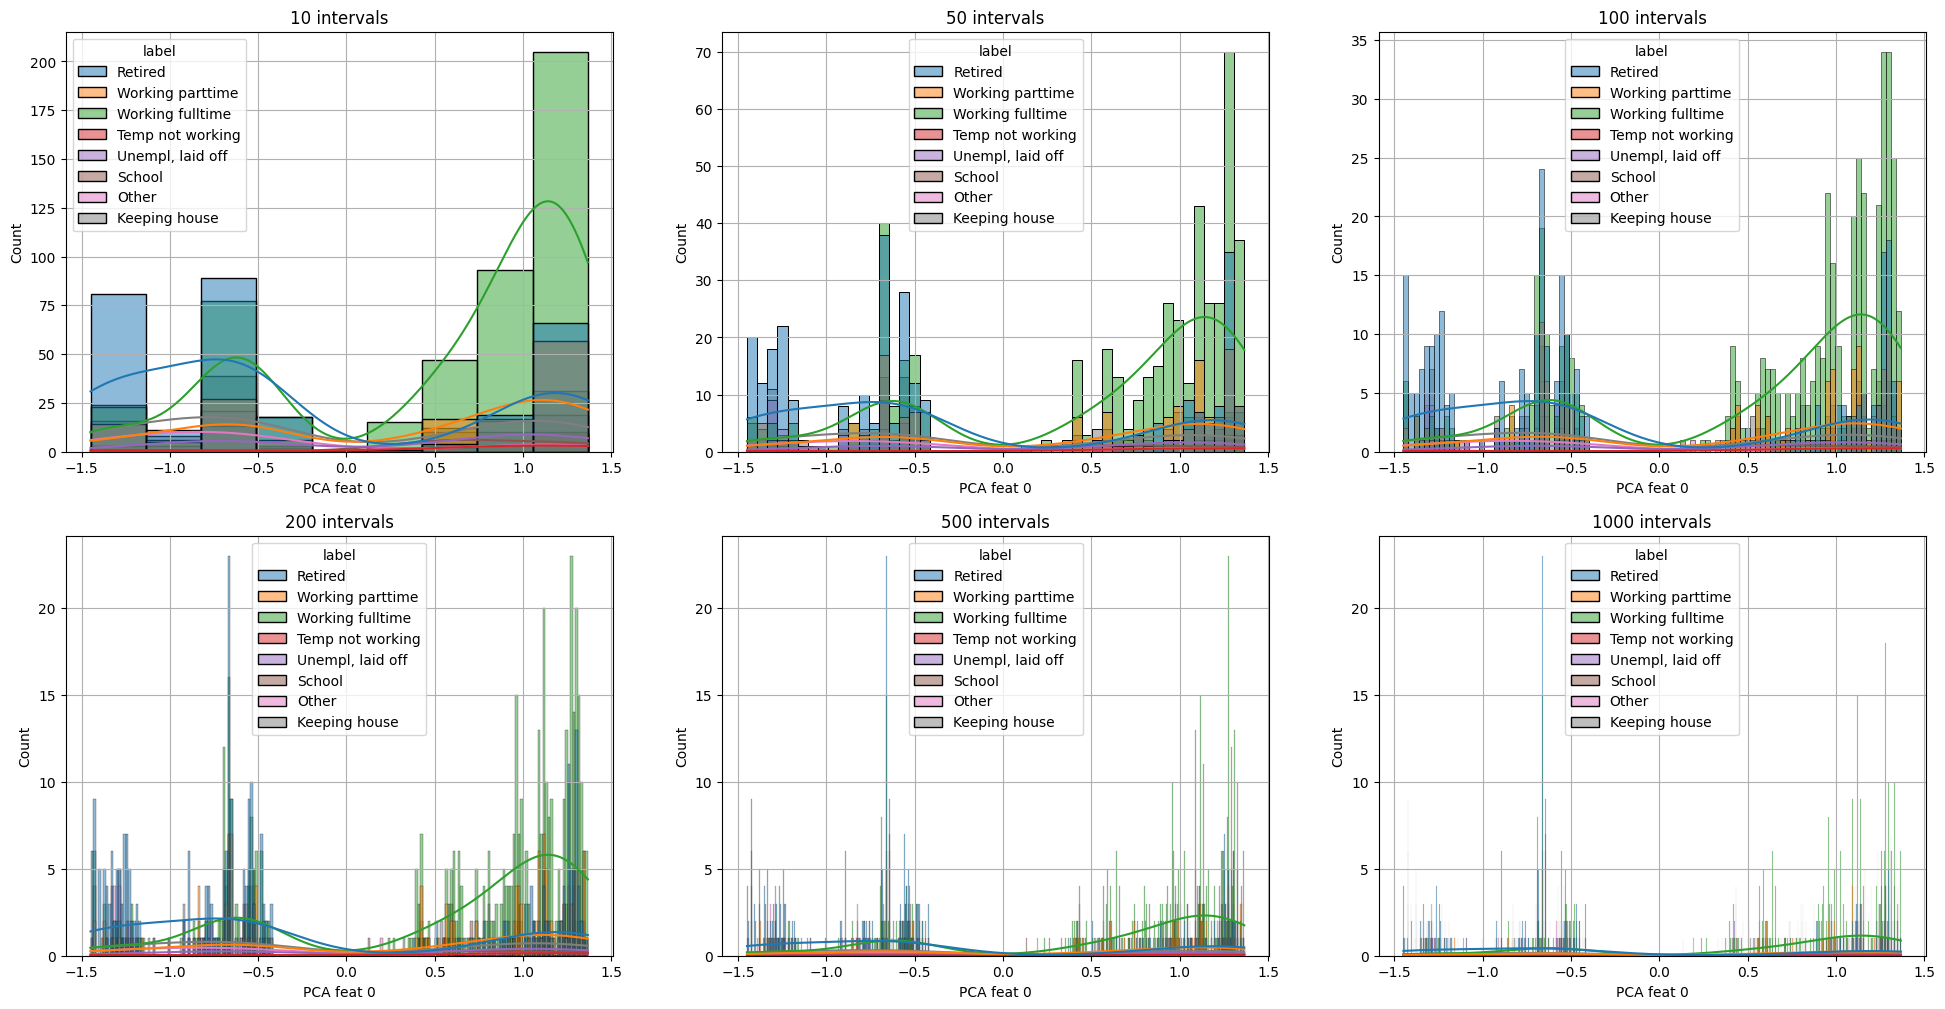
\includegraphics[width=0.75\textwidth]{figures/Thanh/Data_Analysis/With_null_histogram_PCA_feature_0_vs_wrkstat_labels.png}
    \caption{Histogram của thành phần chính thứ nhất tương ứng với từng giá trị dữ liệu trong cột trạng thái làm việc wrkstat}
    \label{fig:With_null_histogram_PCA_feature_0_vs_wrkstat_labels}
\end{figure}

Hình \ref{fig:With_null_histogram_PCA_feature_0_vs_wrkstat_labels} biểu diễn histogram của thành phần chính thứ nhất tương ứng với từng giá trị dữ liệu trong cột trạng thái làm việc wrkstat.
Ta nhận thấy một điều phân phối của histogram của thành phần chính thứ nhất theo các nhóm tương ứng với giá trị trong cột wrkstat gần như cùng hình dạng và trộn lẫn hoàn toàn vào nhau.
Các phân phối cùng đạt cực đại hoặc cực tiểu tại các giá trị trên trục hoành gần như trung nhau.
Ta gần như không nhận thấy sự khác biệt nào về phân phối của thành phần chính thứ nhất theo các nhóm giá trị trong cột wrkstat.

\begin{figure}[H]
    \centering
    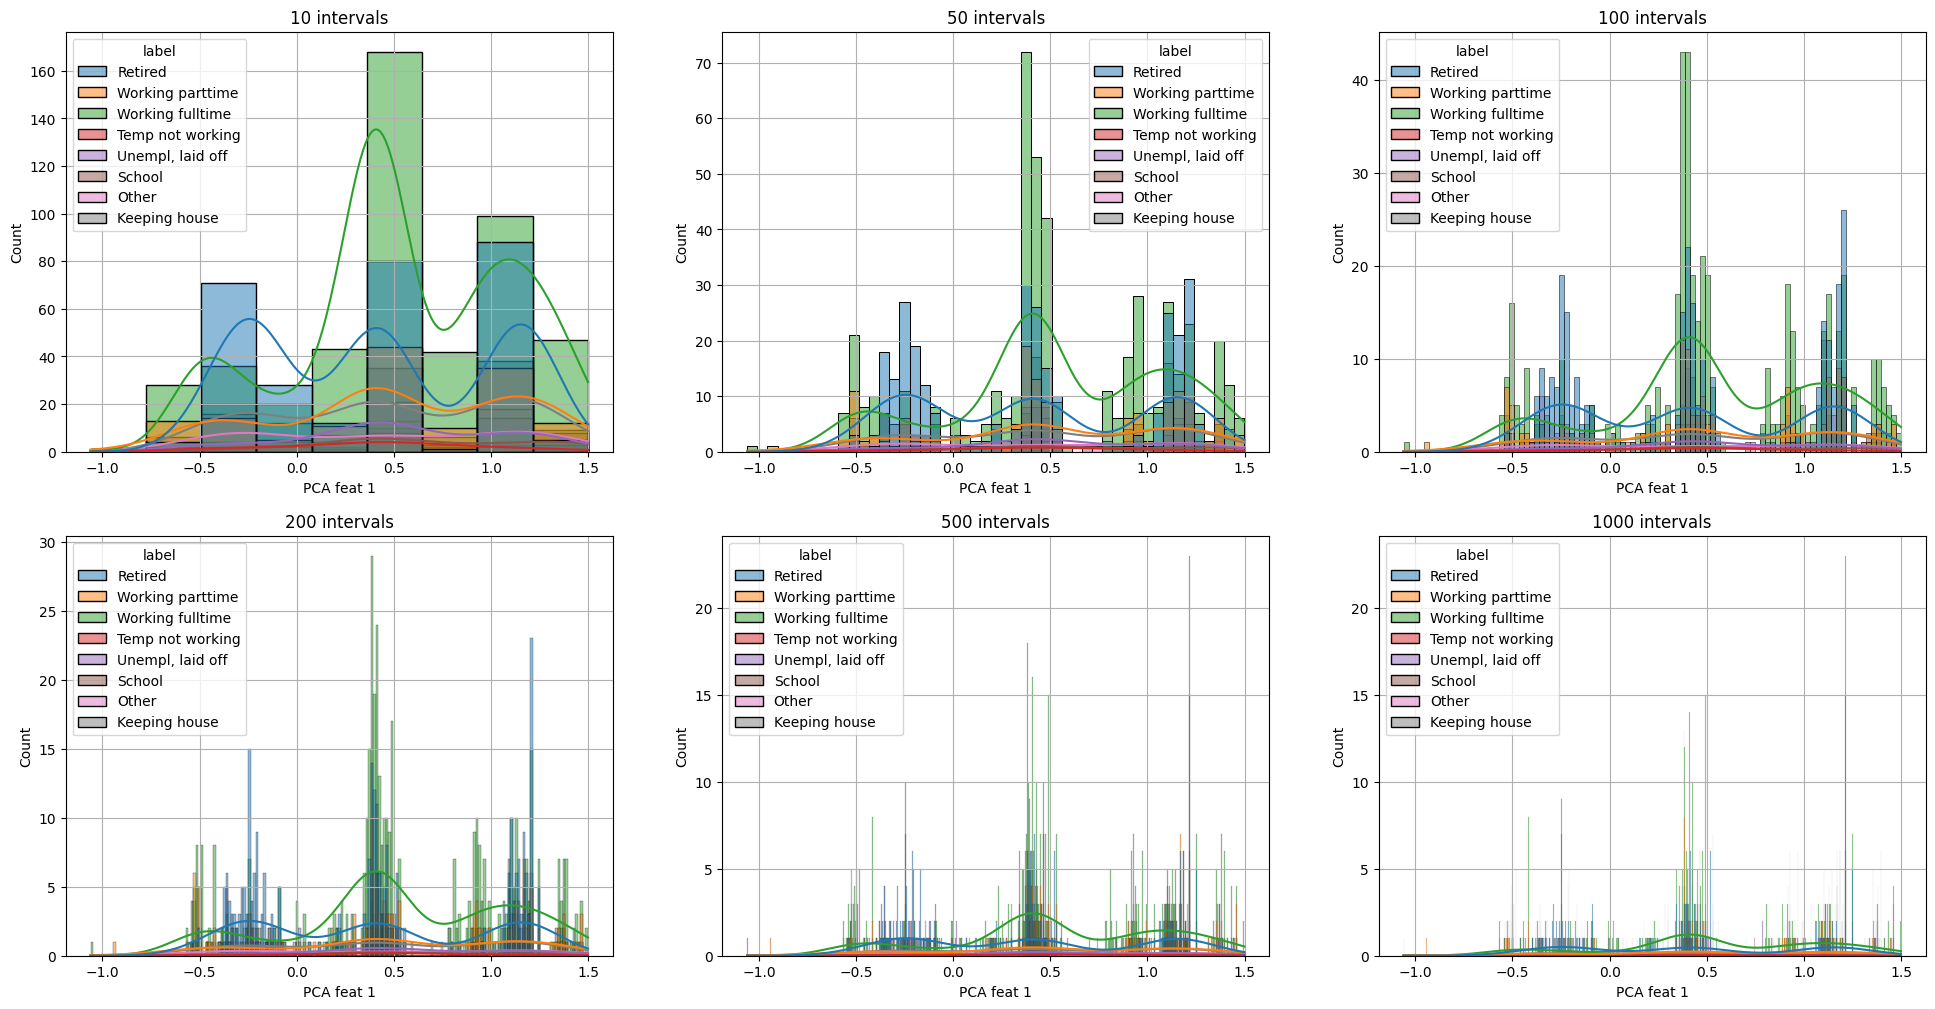
\includegraphics[width=0.75\textwidth]{figures/Thanh/Data_Analysis/With_null_histogram_PCA_feature_1_vs_wrkstat_labels.png}
    \caption{Histogram của thành phần chính thứ hai tương ứng với từng giá trị dữ liệu trong cột trạng thái làm việc wrkstat}
    \label{fig:With_null_histogram_PCA_feature_1_vs_wrkstat_labels}
\end{figure}

\begin{figure}[H]
    \centering
    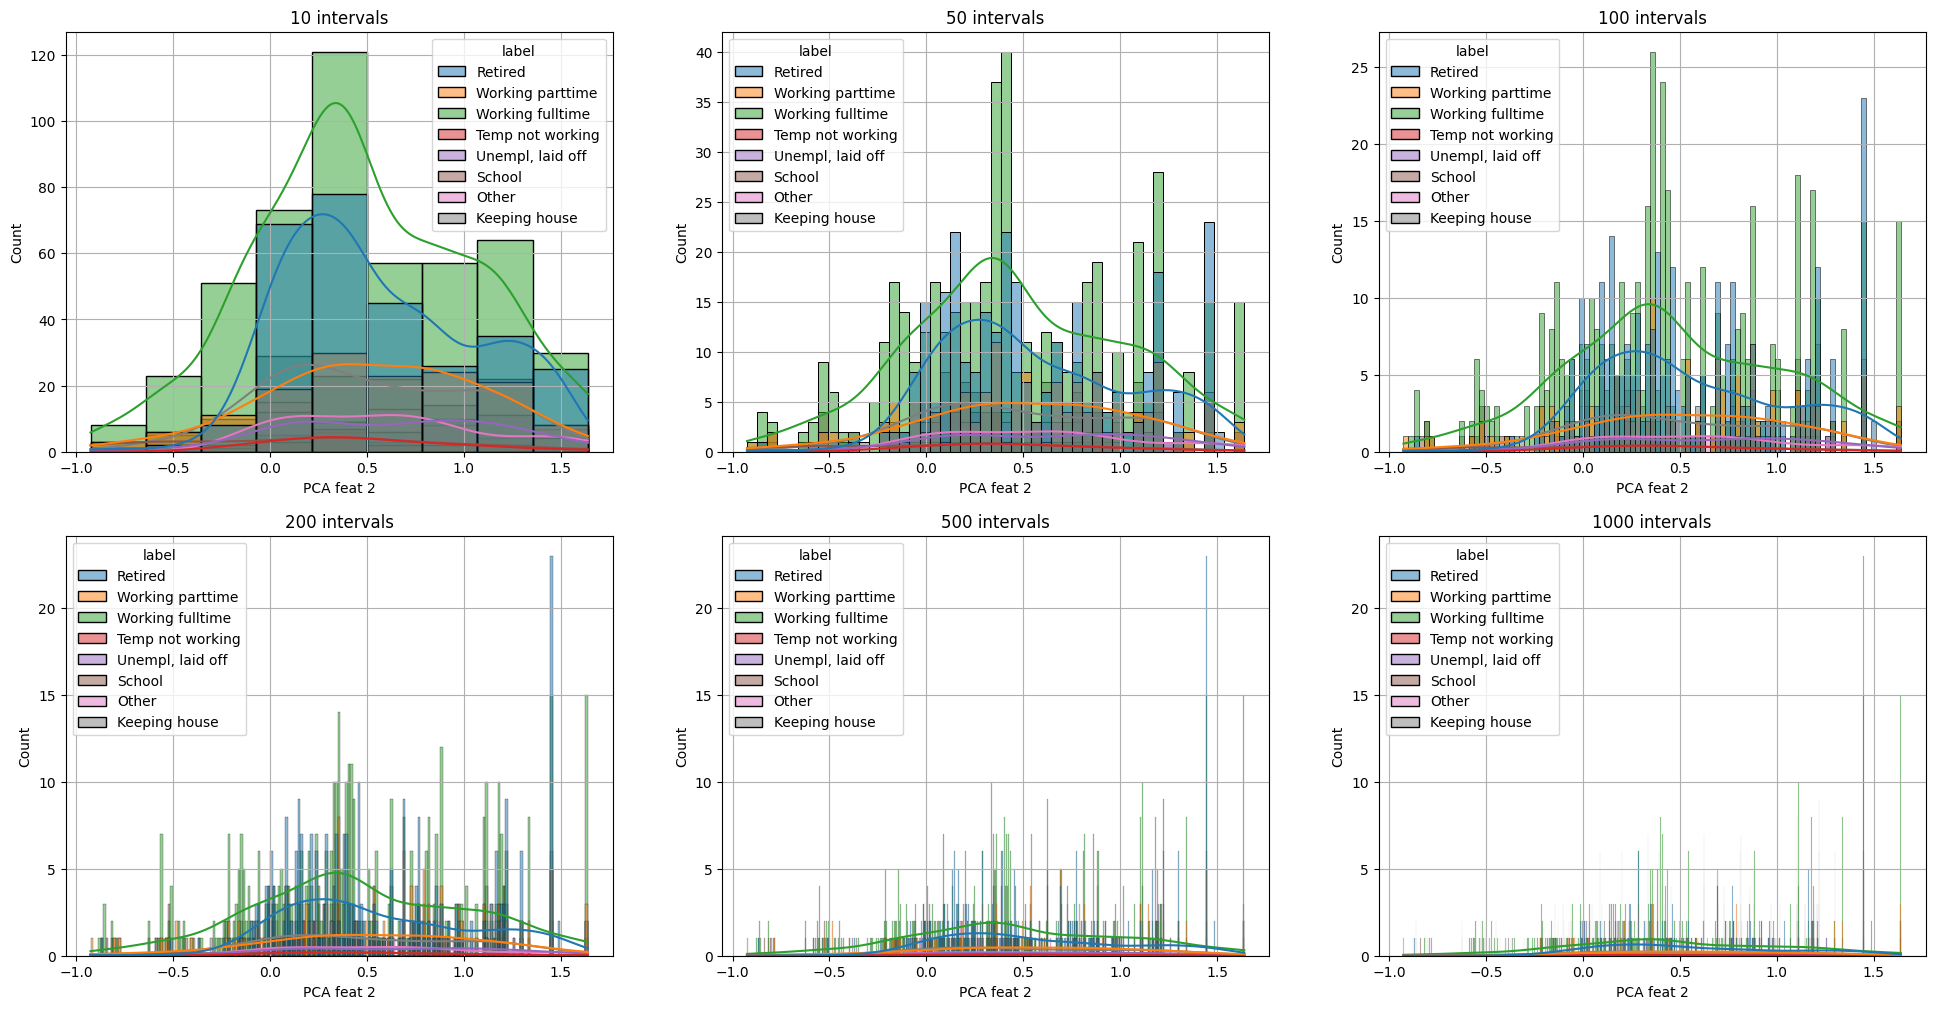
\includegraphics[width=0.75\textwidth]{figures/Thanh/Data_Analysis/With_null_histogram_PCA_feature_2_vs_wrkstat_labels.png}
    \caption{Histogram của thành phần chính thứ ba tương ứng với từng giá trị dữ liệu trong cột trạng thái làm việc wrkstat}
    \label{fig:With_null_histogram_PCA_feature_2_vs_wrkstat_labels}
\end{figure}


Hình \ref{fig:With_null_histogram_PCA_feature_1_vs_wrkstat_labels} và hình \ref{fig:With_null_histogram_PCA_feature_2_vs_wrkstat_labels} biểu diễn histogram của thành phần chính thứ hai và thứ ba tương ứng với từng giá trị dữ liệu trong cột trạng thái làm việc wrkstat.
Ta thấy hiện tượng tương tự cũng xảy ra với hai thành phần chính thứ hai và thứ ba là phân phối của histogram của các thành phần chính theo các nhóm tương ứng với giá trị trong cột wrkstat gần như cùng hình dạng và trộn lẫn hoàn toàn vào nhau.

Đây là điều rất không mong đợi đối với dữ liệu trong các bài toán phân loại.
Do không thể thấy sự khác biệt về phân phối giữa các nhãn dữ liệu tương ứng, ta rất khó có thể xây dựng một mô hình phân loại tốt.

\begin{figure}[H]
    \centering
    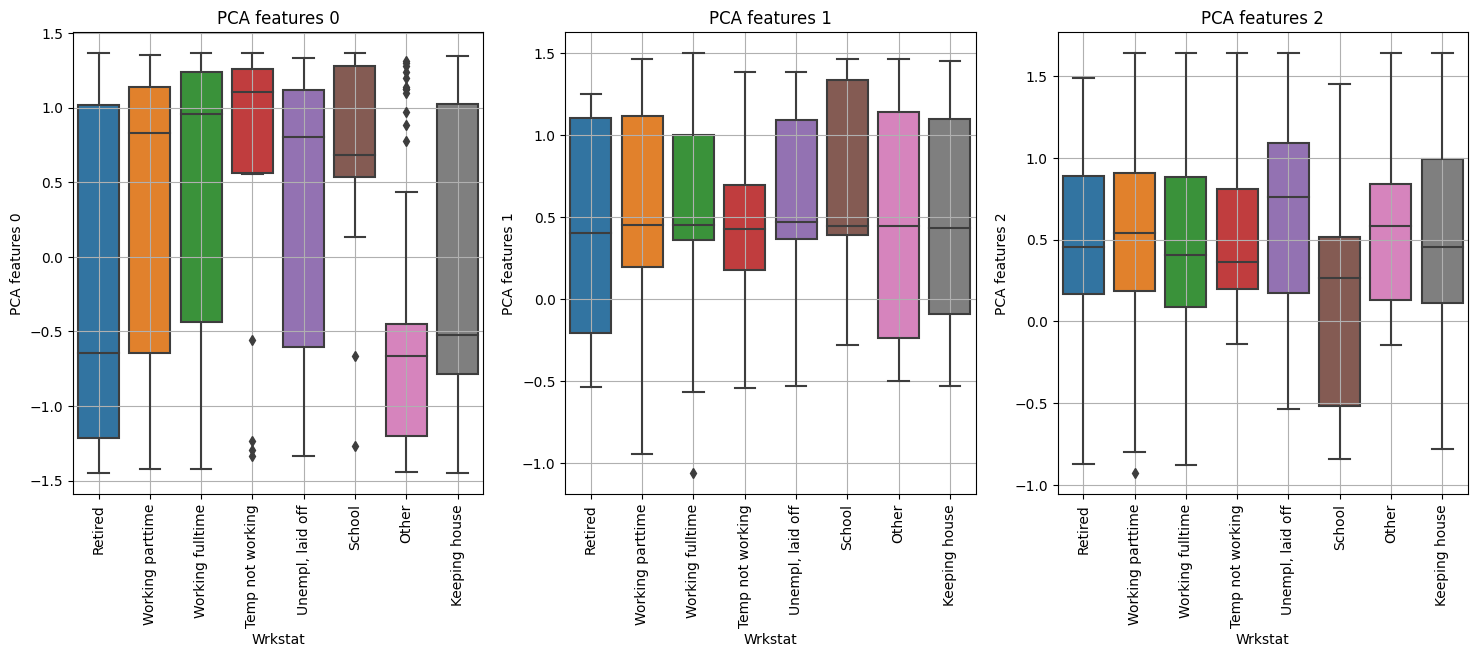
\includegraphics[width=0.8\textwidth]{figures/Thanh/Data_Analysis/With_null_boxplot_PCA_features_vs_wrkstat_labels.png}
    \caption{Boxplot của các thành phần chính tương ứng với từng giá trị trong cột wrkstat}
    \label{fig:With_null_boxplot_PCA_features_vs_wrkstat_labels}
\end{figure}

Hình \ref{fig:With_null_boxplot_PCA_features_vs_wrkstat_labels} thể hiện boxplot của các thành phần chính tương ứng với từng giá trị trong cột wrkstat.
Ta vẫn nhận thấy phân phối của các thành phần chính tương ứng với các nhãn trong cột wrkstat là không có sự tách biệt rõ ràng.
Trừ nhãn Other có phân phối tương ứng với thành phần chính thứ nhất tương đối tách biệt so với phân phối tương ứng với thành phần chính thứ nhất của các nhãn còn lại.

\begin{figure}[H]
    \centering
    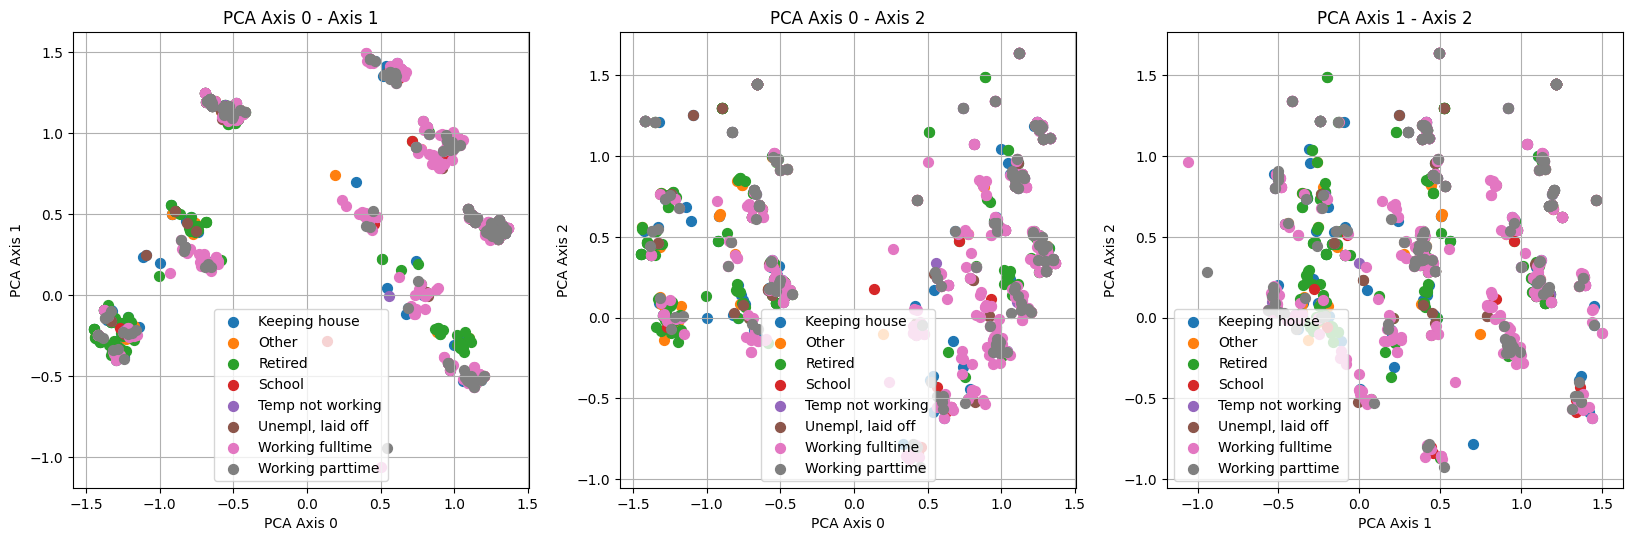
\includegraphics[width=0.8\textwidth]{figures/Thanh/Data_Analysis/With_null_scatterplot_couples_of_PCA_features_vs_wrkstat_labels.png}
    \caption{Scatter plot của các điểm dữ liệu theo các thành phần chính, màu sắc thể hiện giá trị của cột wrkstat}
    \label{fig:With_null_scatterplot_couples_of_PCA_features_vs_wrkstat_labels}
\end{figure}

Hình \ref{fig:With_null_scatterplot_couples_of_PCA_features_vs_wrkstat_labels} biểu diễn scatter plot của các điểm dữ liệu theo các thành phần chính, màu sắc thể hiện giá trị của cột wrkstat.
Ta nhận thấy các quan sát tập trung thành tám, chín nhóm nhỏ.
Các nhóm này có dạng hình cầu.
Một điều không may mắn là trong các nhóm này thì gần như nhóm nào cũng có sự góp mặt của tất cả các quan sát đến từ các nhãn trong cột wrkstat.

Ta thực hiện phân cụm các quan sát.
Hình dạng các nhóm có dạng hình cầu, K-Means phù hợp trong trường hợp này.
Nhưng để thống nhất với trường hợp tập dữ liệu trước, ta vẫn sử dụng thuật toán DBSCAN.

\begin{figure}[H]
    \centering
    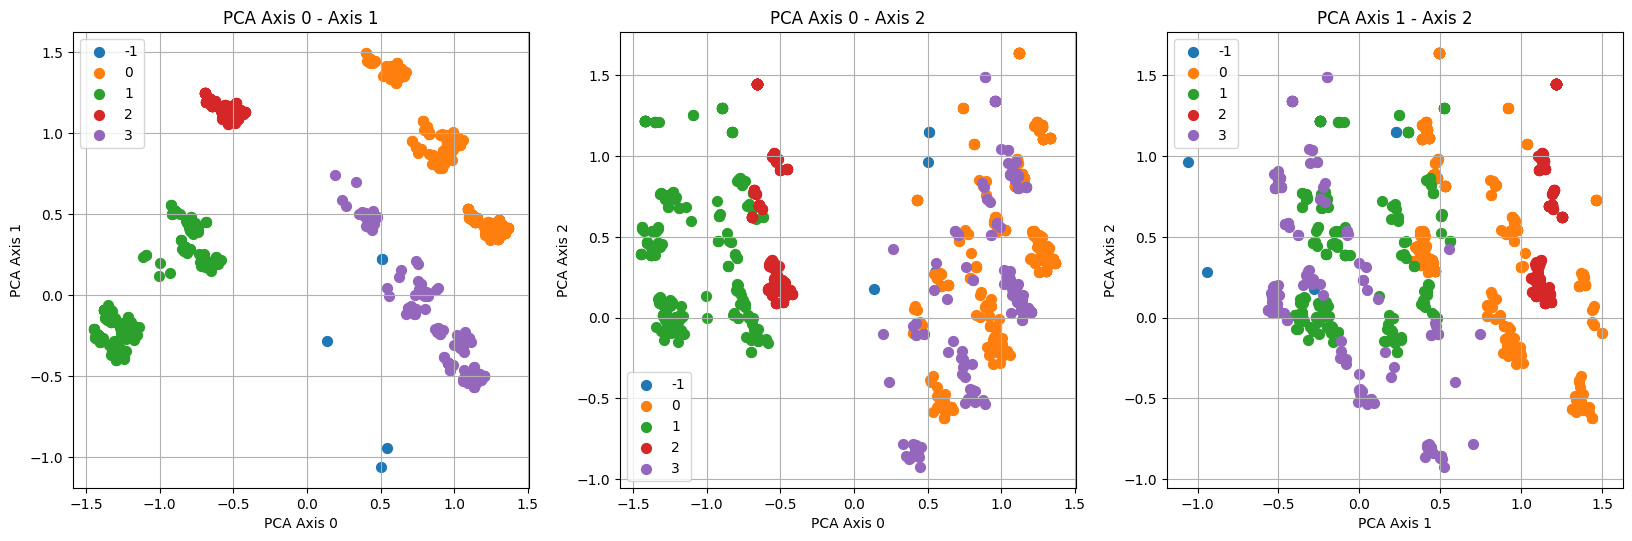
\includegraphics[width=0.8\textwidth]{figures/Thanh/Data_Analysis/With_null_scatterplot_couples_of_PCA_features_vs_pseudo_clustering_labels.png}
    \caption{Scatter plot của các điểm dữ liệu theo các thành phần chính, màu sắc thể hiện các cụm mà các quan sát được gán vào}
    \label{fig:With_null_scatterplot_couples_of_PCA_features_vs_pseudo_clustering_labels}
\end{figure}

Hình \ref{fig:With_null_scatterplot_couples_of_PCA_features_vs_pseudo_clustering_labels} thể hiện Scatter plot của các điểm dữ liệu theo các thành phần chính, màu sắc thể hiện các cụm mà các quan sát được gán vào.
Có bốn nhóm lớn có số lượng quan sát đều khá lớn là nhóm 0, 1, 2, 3.
Các quan sát còn lại không thuộc bốn nhóm trên đều là nhóm -1 được xem là các điểm ngoại lai.
Ta sẽ xem các nhóm là kết quả của quá trình phân cụm là các nhãn giả và thử một số mô hình phân loại và đánh giá hiệu quả của các mô hình trên tương ứng với các nhãn giả này.

Ta sẽ sử dụng hai loại biểu diễn là các vector ban đầu và các vector được phân tích thành phần chính sử dụng thuật toán PCA từ các vector ban đầu của các quan sát.
Ta sẽ thử ba mô hình phân loại là mô hình Multinomial Logistic Regression, Random Forest và AdaBoost.
Ta chia tập dữ liệu với tỷ lệ 0.6 cho tập train và 0.4 cho tập test.
Ta phân chia theo chiến lược stratify sampling để bảo toàn tỷ lệ của các nhãn trong cả tập train và tập test.

\subsubsection{Multinomial Logistic Regression}

\begin{enumerate}[label=(\alph*)]
    \item Đầu vào là vector thu được từ phân tích thành phần chính sử dụng thuật toán PCA 
    
    Ta có bảng kết quả huấn luyện mô hình:

    \begin{python}
        precision    recall  f1-score   support

          -1       0.00      0.00      0.00         4
           0       1.00      1.00      1.00       211
           1       1.00      1.00      1.00       102
           2       1.00      1.00      1.00        99
           3       0.94      1.00      0.97        68

    accuracy                           0.99       484
   macro avg       0.79      0.80      0.79       484
weighted avg       0.98      0.99      0.99       484
    \end{python}

    và ma trận nhầm lẫn:

    \begin{figure}[H]
        \centering
        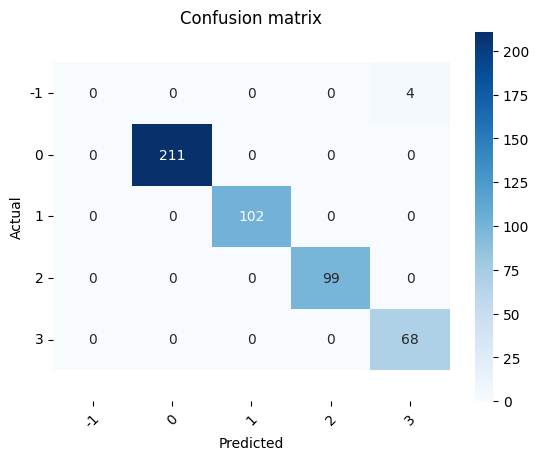
\includegraphics[width=0.6\textwidth]{figures/Thanh/Data_Analysis/With_null_confusion_matrix_Logistic_PCA_features.png}
        \caption{Ma trận nhầm lẫn của mô hình Multinomial Logistic Regression khi vector đầu vào được phân tích thành phần chính}
        \label{fig:With_null_confusion_matrix_Logistic_PCA_features}
    \end{figure}

    Kết quả phân loại của mô hình rất tốt.
    Trừ nhãn giả -1, tất cả các nhãn giả khác đều có độ hồi tưởng là 1.

    Ta sẽ phân tích ngược trở lại trọng số của các tham số tương ứng với các đặc trưng của vector ban đầu từ các tham số ứng với các đặc trưng của các thành phần chính.

    \begin{figure}[H]
        \centering
        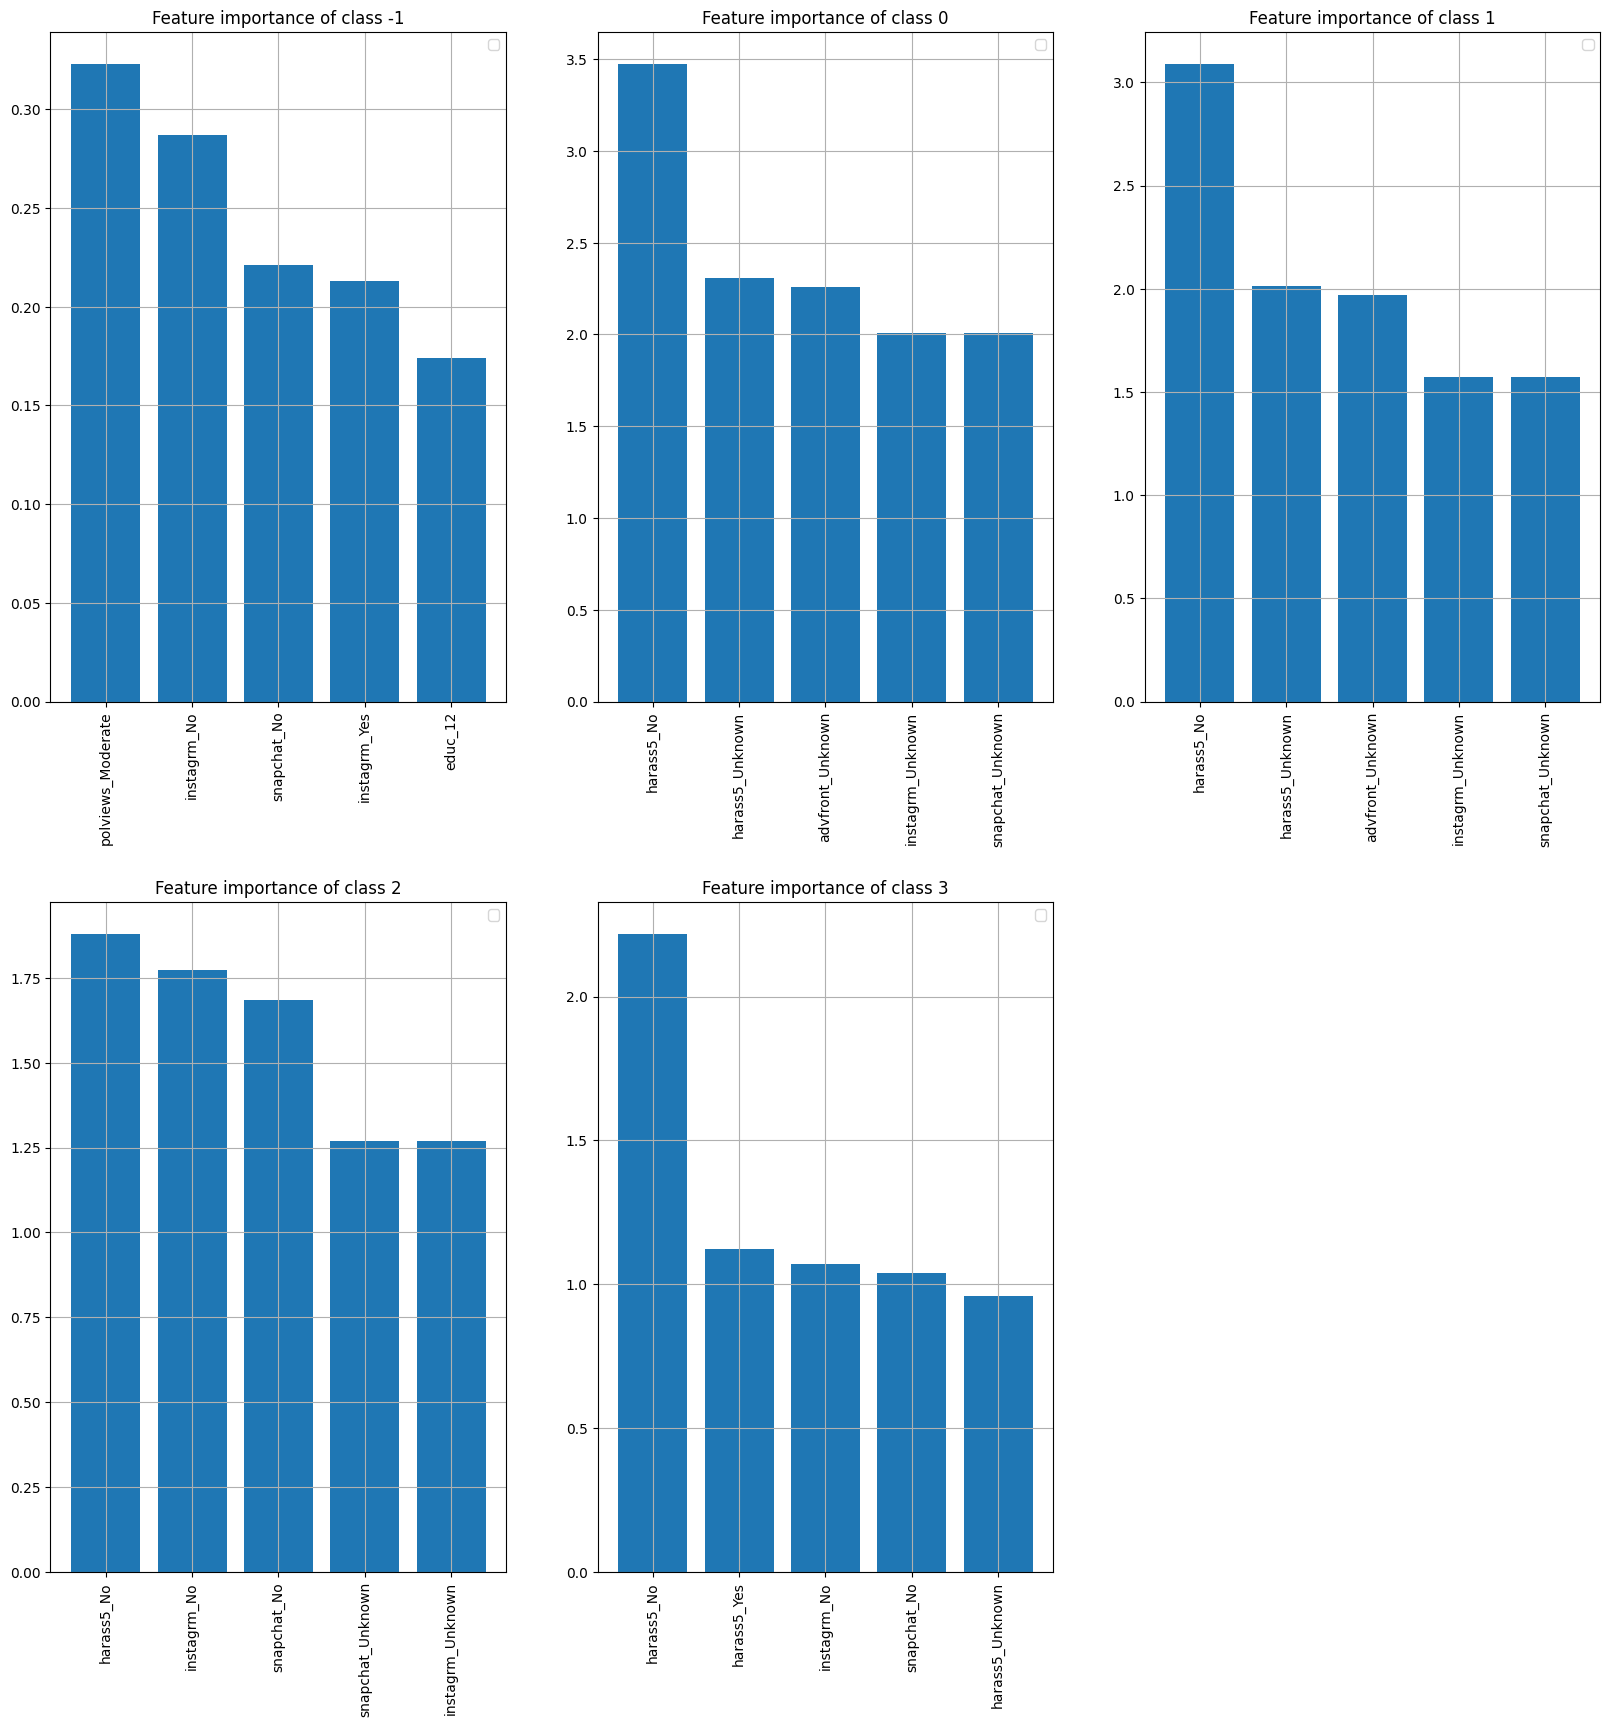
\includegraphics[width=0.6\textwidth]{figures/Thanh/Data_Analysis/With_null_Feature_Importance_Logistic_PCA_features.png}
        \caption{Biểu đồ cột sắp xếp độ lớn giảm dần (trị tuyệt đối) tham số của các đặc trưng ứng với từng nhãn giả}
        \label{fig:With_null_Feature_Importance_Logistic_PCA_features}
    \end{figure}

    Ta có biểu đồ cột sắp xếp độ lớn giảm dần (trị tuyệt đối) tham số của các đặc trưng ứng với từng nhãn giả thể hiện ở hình \ref{fig:With_null_Feature_Importance_Logistic_PCA_features}.
    Ta nhận thấy các đặc trưng tương ứng với harass5\_No, instagrm\_No, harass5\_Unknown, snapchat\_No có trọng số khá lớn.
    Ta nhận thấy đặc điểm chung của các đặc trưng này là tần suất của các giá trị tương ứng với các đặc trưng trên lớn (hình \ref{fig:With_null_frequency_of_unique_values_of_columns})

    \begin{figure}[H]
        \centering
        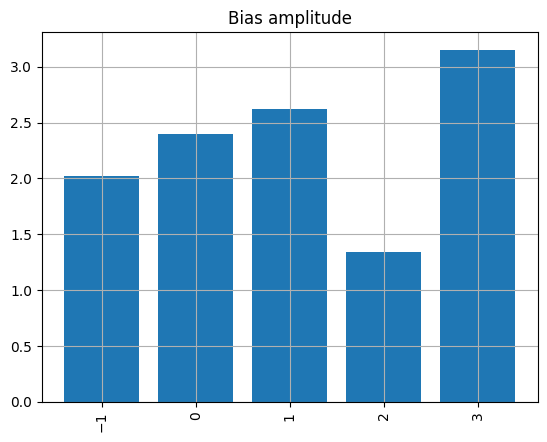
\includegraphics[width=0.6\textwidth]{figures/Thanh/Data_Analysis/With_null_Bias_Importance_Logistic_PCA_features.png}
        \caption{Biểu đồ cột thể hiện độ lớn của các bias tương ứng với từng nhãn giả}
        \label{fig:With_null_Bias_Importance_Logistic_PCA_features}
    \end{figure}

    Hình \ref{fig:With_null_Bias_Importance_Logistic_PCA_features} thể hiện độ lớn của các bias tương ứng với từng nhãn giả.

    \item Vector đầu vào là vector gốc ban đầu
    
    Ta có bảng kết quả huấn luyện mô hình:

    \begin{python}
        precision    recall  f1-score   support

        -1       0.00      0.00      0.00         4
         0       1.00      1.00      1.00       211
         1       1.00      1.00      1.00       102
         2       1.00      1.00      1.00        99
         3       0.94      1.00      0.97        68

  accuracy                           0.99       484
 macro avg       0.79      0.80      0.79       484
weighted avg       0.98      0.99      0.99       484
    \end{python}

    và ma trận nhầm lẫn:

    \begin{figure}[H]
        \centering
        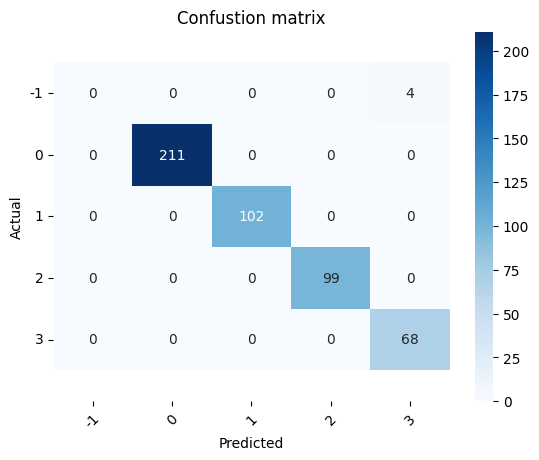
\includegraphics[width=0.6\textwidth]{figures/Thanh/Data_Analysis/With_null_confusion_matrix_Logistic_original_features.png}
        \caption{Ma trận nhầm lẫn của mô hình Multinomial Logistic Regression khi vector đầu vào là vector gốc ban đầu}
        \label{fig:With_null_confusion_matrix_Logistic_original_features}
    \end{figure}

    Ta nhận thấy kết quả phân loại trùng hoàn toàn so với trường hợp đầu vào là vector đã được phân tích thành phần chính sử dụng thuật toán PCA.

    Ta sẽ phân tích ngược trở lại trọng số của các tham số tương ứng với các đặc trưng của vector ban đầu từ các tham số ứng với các đặc trưng của các thành phần chính:

    \begin{figure}[H]
        \centering
        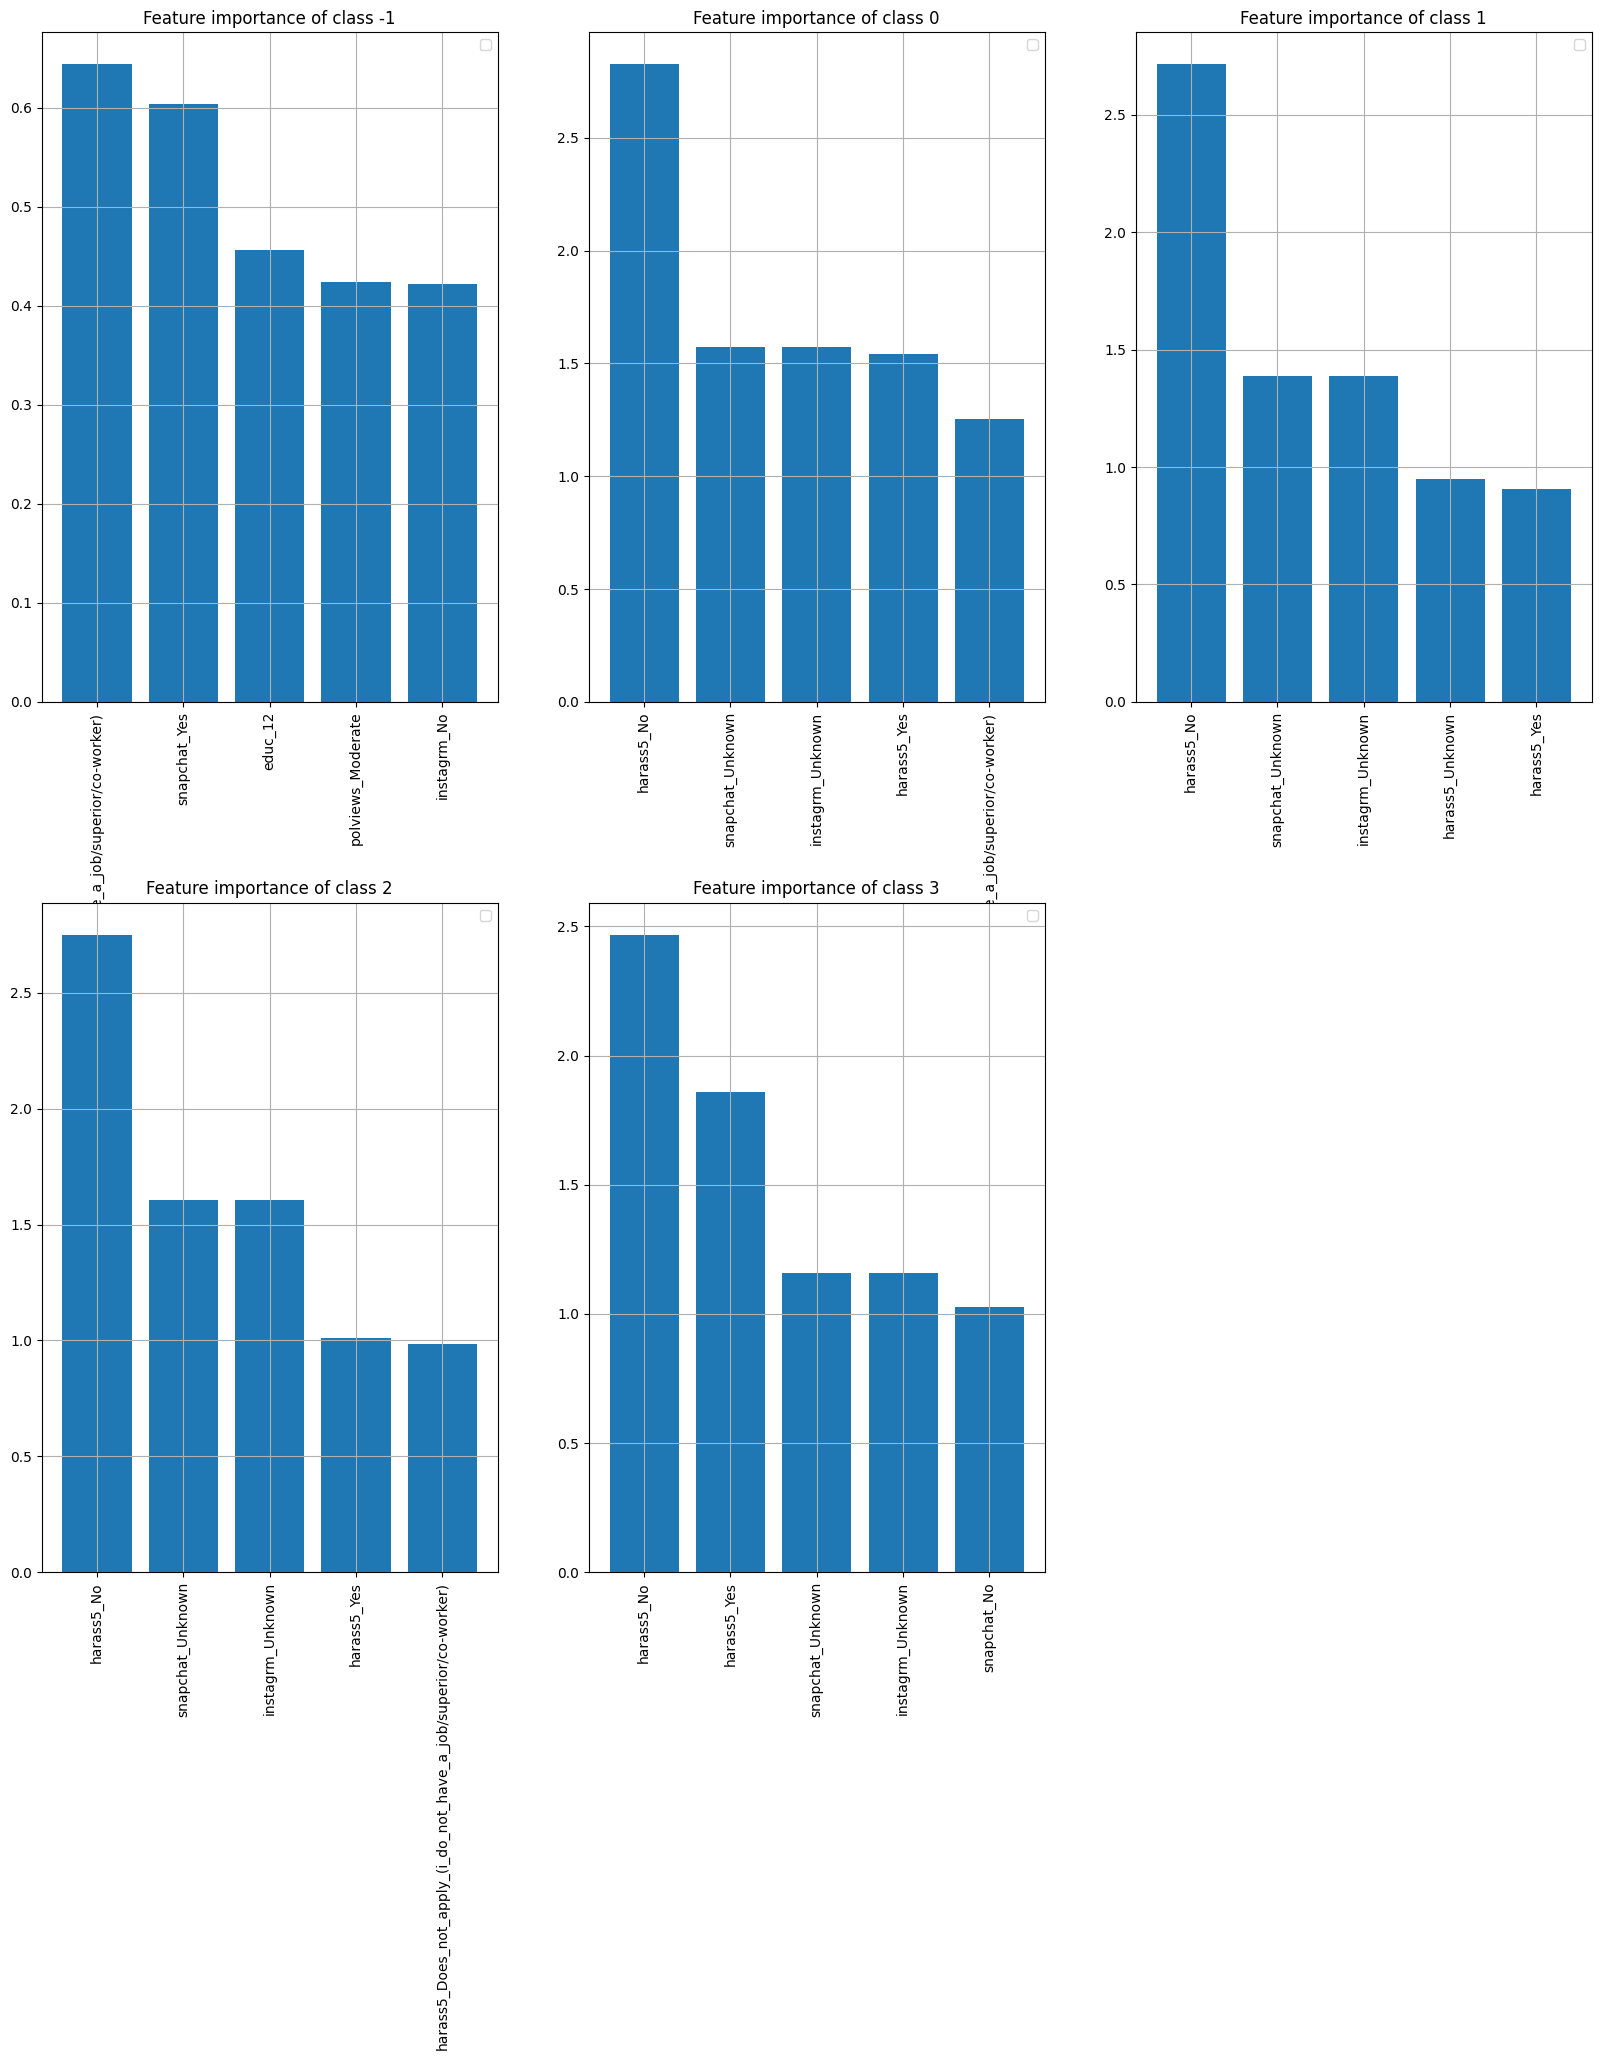
\includegraphics[width=0.6\textwidth]{figures/Thanh/Data_Analysis/With_null_Feature_Importance_Logistic_original_features.png}
        \caption{Biểu đồ cột sắp xếp độ lớn giảm dần (trị tuyệt đối) tham số của các đặc trưng ứng với từng nhãn giả (mô hình với vector đầu vào là vector gốc ban đầu)}
        \label{fig:With_null_Feature_Importance_Logistic_original_features}
    \end{figure}

    Ta có biểu đồ cột sắp xếp độ lớn giảm dần (trị tuyệt đối) tham số của các đặc trưng ứng với từng nhãn giả thể hiện ở hình \ref{fig:With_null_Feature_Importance_Logistic_original_features}.
    Các đặc trưng có trọng số lớn vẫn là các đặc trưng có trọng số lớn ở trường hợp trước khi vector đầu vào là vector được phân tích thành phần chính: harass5\_No, snapchat\_Unknown, instagrm\_Unknown.
    Lý do có thể là vì tần suất của các giá trị harass5\_No, snapchat\_Unknown, instagrm\_Unknown có tần suất cao trong tập dữ liệu (hình \ref{fig:With_null_frequency_of_unique_values_of_columns}).

    \begin{figure}[H]
        \centering
        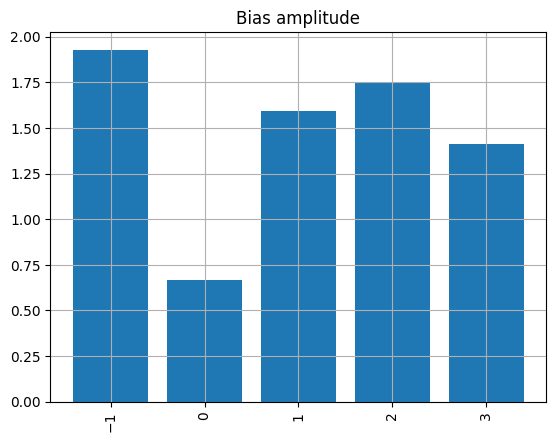
\includegraphics[width=0.6\textwidth]{figures/Thanh/Data_Analysis/With_null_Bias_Importance_Logistic_original_features.png}
        \caption{Biểu đồ cột thể hiện độ lớn của các bias tương ứng với từng nhãn giả (mô hình với vector đầu vào là vector gốc ban đầu)}
        \label{fig:With_null_Bias_Importance_Logistic_original_features}
    \end{figure}

    Hình \ref{fig:With_null_Bias_Importance_Logistic_original_features} thể hiện độ lớn của các bias tương ứng với từng nhãn giả.
    Kết quả thể hiện ngược lại với trường hợp vector đầu vào là vector được phân tích thành phần chính sử dụng thuật toán PCA từ vector gốc ban đầu.
    Nhãn giả 2 trường hợp đầu vào là vector được phân tích thành phần chính có bias tương đối nhỏ nhưng với trường hợp đầu vào là vector gốc ban đầu thì bias tương đối lớn

\end{enumerate}